\section{Genomics}
The field of genomics is closely related to, yet distinct, from the field of genetics, which itself stems from the work of such seminal figures as Charles Darwin\autocite{originofspecies} and Gregor Mendel\autocite{mendel1865}. While genetics largely focuses on the study of single (or relatively small numbers of) genes - the \emph{genotype}, and how genetic variation and mutation affect the physical traits of a given cell or organism - its \emph{phenotype}, genomics focuses on larger scale events and mechanisms that tend to act on the entirety of an organism's genome, shaping its architecture and ultimately affecting its survival.

\subsection{History of Genomics}
Each living cell is a bio-chemical machine that carries out a number of complex behaviours such as interactions with the surrounding environment, motility, metabolism, and reproduction, that are necessary for its survival and proliferation, based on a genetic program that is encoded within the cell's DNA. The DNA is nominally subdivided into functionally distinct areas known as \emph{genes}. The cell utilizes the program within each gene by first \emph{transcribing} the DNA into an intermediary information-carrier molecule called RNA, and then \emph{translating} this RNA into molecules called \emph{proteins} that are utilized by the cell to carry out the majority of its functions. Understanding and interpretation of the underlying genetic program thus underpins our ability to comprehend the entirety of the different behaviours that each cell undertakes.

The success of this undertaking is contingent, first and foremost, on our ability to effectively read off the information encoded in the DNA, an activity known as \emph{sequencing}. We are able to sequence DNA thanks to the pioneering work of researchers Rosalind Franklin\autocite{franklin1953molecular}, James Watson, and Francis Crick\autocite{watson1953molecular} who first elucidated the physical structure of DNA, then followed by the work of Fred Sanger\autocite{sanger1977dna,sanger1975rapid} who devised the first effective DNA sequencing method. The sequencing method allows us to transform information that is physically encoded on the DNA molecule via a sequence of four distinct types of \emph{basepairs} - Adenine, Cytosine, Guanine, and Thymine into a string stored on a computer using a four-letter alphabet - A,C,T, and G, thus turning DNA interpretation into a digital information processing problem.

While the entire length of the DNA of an organism ranges from several hundred thousand basepairs for simple organisms like viruses and bacteria, to about 3,000,000,000 basepairs for a human, to over 150,000,000,000 for certain plants\autocite{pellicer2010largest} the limitations of Sanger DNA sequencing technology are such that the sequencing machine can only produce DNA fragment strings, known as \emph{reads} that are 800 - 1,000 basepairs long\autocite{sanger1977dna}. Reconstituting the original complete DNA sequence from partial overlaps between reads is thus a costly, time consuming, and computationally intensive problem known as \emph{de-novo assembly}\autocite{zerbino2008velvet}. Once one such full sequence (known as a \emph{reference} sequnce) is assembled however, sequencing other individuals of the same (or closely related) species becomes a significantly easier undertaking. Rather than assembling the sequence \emph{de-novo} one can search for a position on the reference sequence that provides the best matching \emph{alignment} between the reference and each read obtained for the specimen under study. This technique is known as \emph{genomic alignment}\autocite{li2009fast} or \emph{mapping} and yields for each fragment a coordinate that represents where on the reference sequence the fragment maps to. Furthermore, because the DNA of any two organisms of the same species is largely identical, with differences occurring at about 0.1\% of all sites (although this depends on DNA mutation rate)\autocite{nachman2001single} researchers are able to significantly reduce the amount of information that is required to fully represent the genome of a specimen by retaining only the information that describes the sites where that specimen is different from the reference sequence for that species. 

A general approach has thus emerged, where each new species of interest undergoes a relatively costly \emph{de-novo} assembly process for the first genome, which then becomes the reference genome for that species. The sequencing of further individuals of that species utilizes, relatively cheaper, \emph{alignment} and identification of \emph{variants} (sites where the individual differs from the reference) to investigate the effect these variants may have on different phenotypes of interest such as disease susceptibility and survival\autocite{manolio2010genomewide}.

Although genomicists study many different types of organisms the study of human genomes garners by far the most attention and research funding\autocite{needcitation} due to the natural desire of humans to better understand ourselves and influence, where possible, genetic factors impacting human longevity and health. Subsequent to the development of DNA sequencing methods by Fred Sanger one of the most audacious and crucial projects for the development of genomics as a branch of science has been The Human Genome Project\autocite{lander2001initial} - an international effort to sequence and \emph{de-novo} assemble the first complete human genome consisting of chromosomes 1-22, X, and Y (as well as mitochondrial DNA) and totalling approximately 3 billion basepairs. The project ran for over 10 years, completing in 2001, and cost more than \$3 billion USD. Although the main project effort was completed using the Sanger sequencing method, a competing version of the human genome was simultaneously published by a commercial company led by JC Venter\autocite{venter2001sequence}, using a new sequencing method called shotgun sequencing\autocite{venter1998shotgun}, a method that formed the basis for a new revolution in sequencing technology, now termed Next Generation Sequencing\autocite{schuster2007next}.

\subsection{Next Generation Sequencing}
The Next Generation Sequencing methodology\autocite{mardis2008next} relies on fragmenting the DNA of a subject into millions of fragments that are between 100-500 basepairs (bp) in length, then sequencing all of the short fragments and aligning all the reads to the reference with the aid of a relatively fast algorithm\autocite{li2010survey}. Because NGS sequencing methods are prone to certain errors and biases\autocite{dohm2008substantial}, it is necessary to sequence enough DNA fragments to overlap (or cover) every location in the genome several times (typically 10-30), in order to build a statistical model that will be able to determine the underlying sequence, known as \emph{genotyping}\autocite{nielsen2011genotype}, with a high degree of confidence. Thus, at present, a single sequenced DNA sample will typically contain 1 billion reads with a file size of ~150GB when compressed.

\begin{figure}[H]
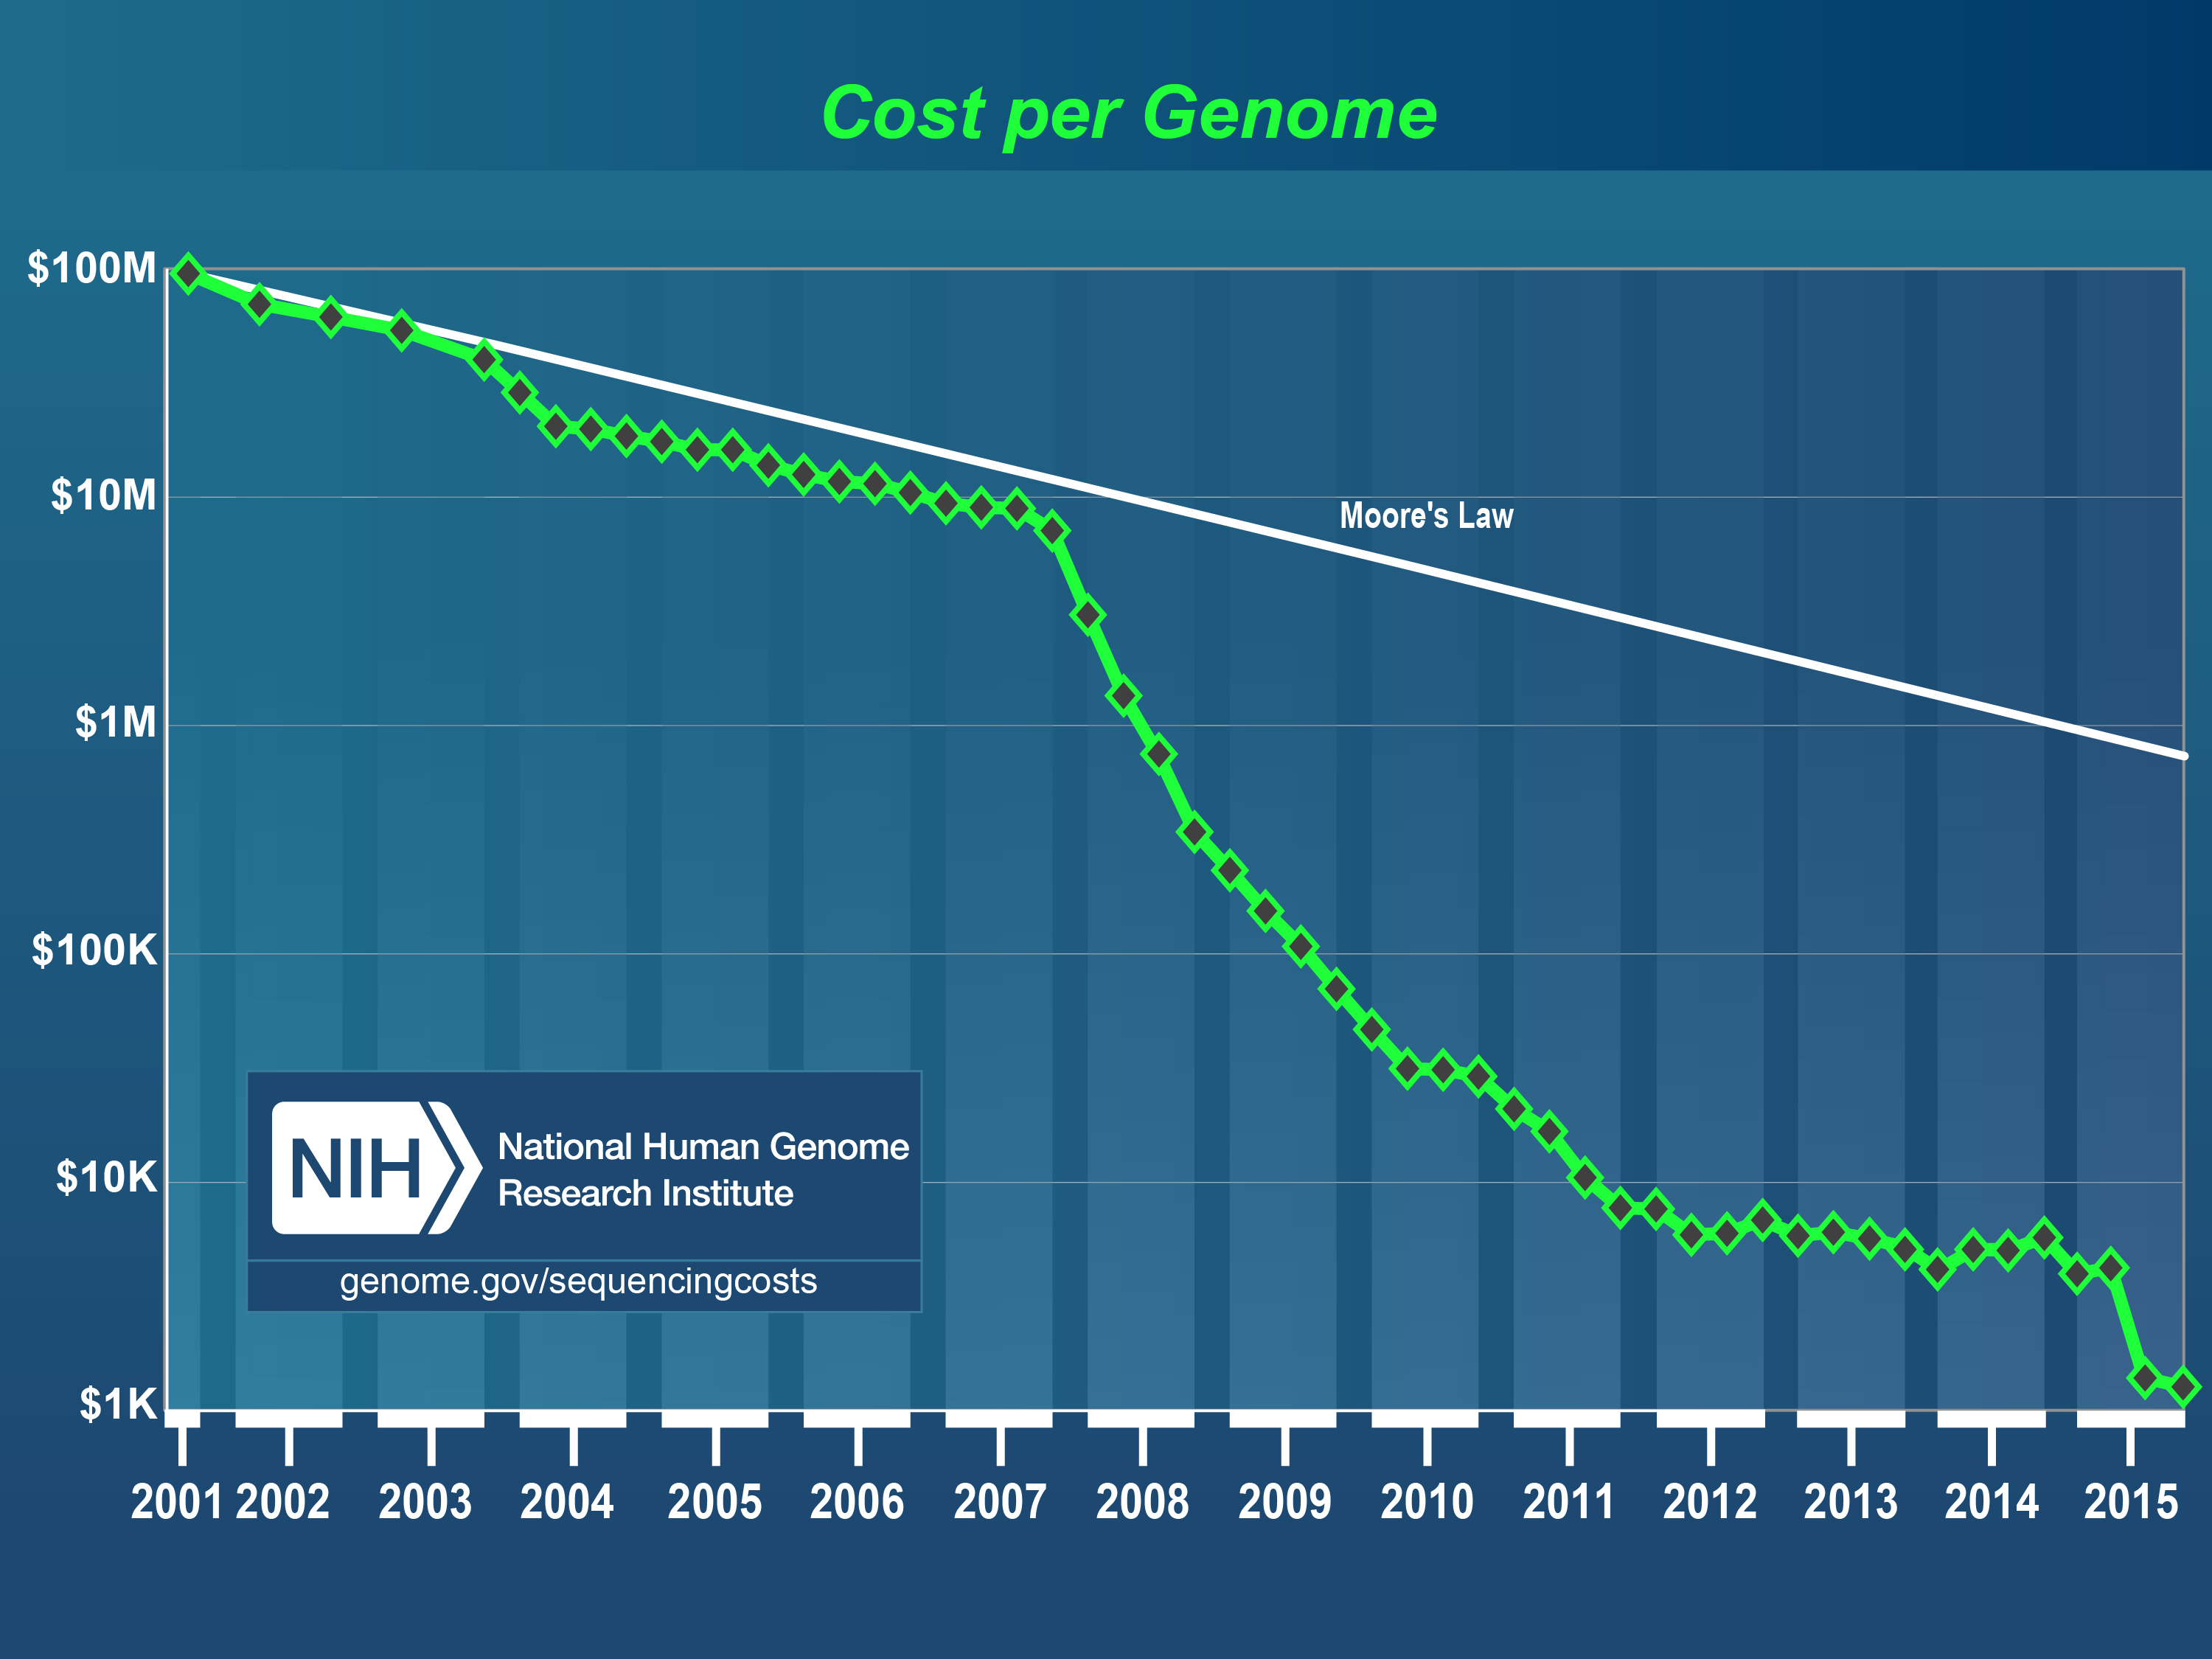
\includegraphics[scale=0.5]{costpergenome2015_4}
\centering
\caption {Cost of DNA sequencing\autocite{The_Cost_of_Sequencing_a_Human_Genome_2016-11-04}}
\label{fig:costpergenome2015_4}
\end{figure}

Figure \ref{fig:costpergenome2015_4} shows the change in the cost of DNA sequencing over the course of the past 15 years. The precipitous drop in sequencing cost observed since 2008 coincides with wide adoption of NGS methodologies. This drop in price has made tractable a new set of large scale genomics sequencing projects that aim to characterize human genetic diversity at population scale, projects such as the 1000 Genomes Project\autocite{10002010map}, and the large scale sequencing of the Icelandic population\autocite{gudbjartsson2015large}.

\subsection{Genomics Studies}

\subsection{Cancer Genomics}
Cancer is a genetic disease that has an extremely high burden on the human population. In 2012, the global incidence of new cases worldwide has been estimated as 14.1 million, and deaths at 8.2 million\autocite{torre2015global}. The economic cost of cancer to the European Union has been estimated at 126 billion euro in 2009\autocite{luengo2013economic}, and in the US \$124.5 billion USD in 2010\autocite{yabroff2011economic}. Because of the genetic nature of the disease studying genomes of cancer patients helps uncover the mechanisms behind the development and evolution of cancer\autocite{stratton2009cancer}.

Cancerous tumours arise from a single cell which over time accumulates a series of somatic mutations that cause it to exhibit properties such as: increased mutation rate, increased proliferation, anchorage independent growth, and resisting cell death\autocite{hanahan2011hallmarks} . Only certain mutations, however, contribute to the development of cancer, while others are benign. Cancer genomics studies aim to identify and characterize those mutations that are cancer drivers and play a role in the formation or progression of tumours\autocite{stratton2009cancer}. 

Studying cancer genomes is more complex and expensive than studying the genomes of healthy individuals because each patient requires that two DNA samples are collected - that of the normal tissue, and that of the tumour. This is necessary to identify those mutations that are somatic - i.e. only occur in the tumour cell population\autocite{roberts2013comparative}.


\begin{figure}[H]
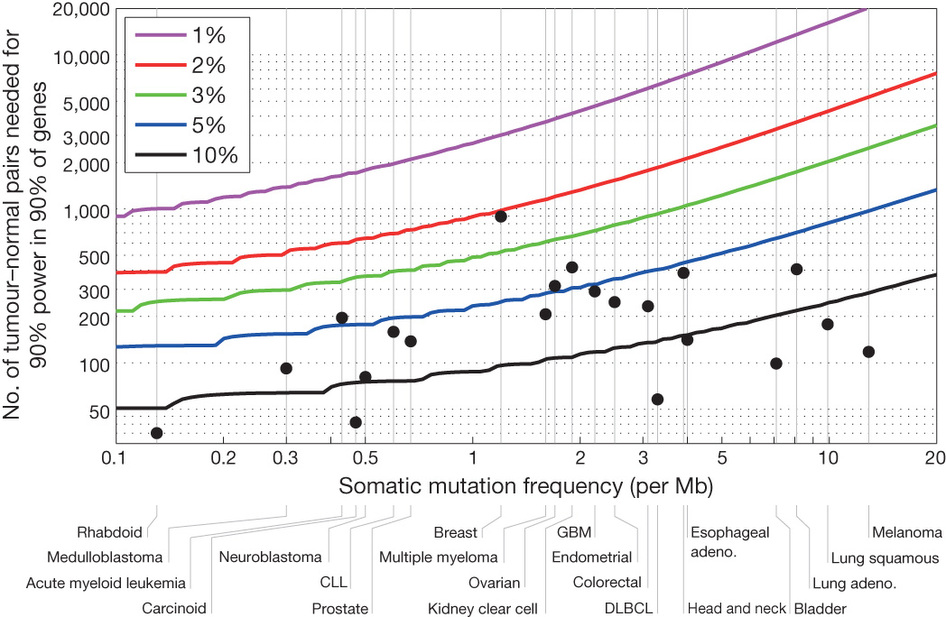
\includegraphics[scale=0.4]{nature12912-f5}
\centering
\caption {Sequencing sample size required by mutation rate\autocite{lawrence2014discovery}.}
\label{fig:nature12912-f5}
\end{figure}

Although there is a large number of identified mutations that are implicated in cancer (2,002,811 SNV,  10,534 gene fusions, 61,299 genome rearrangements, 695,504 CNV segments in COSMIC v70; August 2014)\autocite{forbes2015cosmic}, each mutation has a low chance of being present in any given tumour. Figure \ref{fig:nature12912-f5} demonstrates the sample size required to have 90\% statistical power to identify  90\% of the variants that occur with a set frequency in tumours with varying background mutation rates. Thus, identifying 90\% of the mutations occurring with a frequency of at most 1\% in Lung Adenocarcinoma requires a sample size of at least 10,000 patients. The necessity to sequence large cohorts of patients in order to be able to comprehensively detect  cancer related genomic variants has led to the creation of several large scale cancer sequencing studies.

\subsection{Clinical Genomics}

\section{Computational Methods for Next Generation Sequencing}
Because the size of a typical genome is millions to billions of basepairs long, and current DNA sequencing technology frequently generates errors during the sequencing process, requiring multiple samples of each genomic location to be generated, the amount of data required to be examined in order to characterize even a single sample is well beyond the capabilities of any human. Thus, a multitude of computational approaches are required in order to make the task tractable for individual samples as well as cohorts, and entire populations.

The task of comprehensive characterization of genomic data for an individual is typically decomposed into a series of computational steps, each with its own data representation, and typically developed by a separate research group, which are then assembled into computational pipelines and executed by workflow engines on diverse computing environments. Our goal in this section is to enumerate and describe the individual steps and to provide a survey of the key computational tools and data formats that presently form the set of best practices in this rapidly evolving branch of science. Since Rheos is designed to improve upon these best practices we identify in each section the key mathematical and algorithmic ideas that underpin each approach in order to adapt and translate them into the Rheos framework.

The data that is used in virtually all modern genomics studies is generated on a next generation DNA sequencing machine. Several types of sequencers have been developed but the most frequently used ones are made by Illumina. The raw data produced by such a sequencer is a set of image files, where the color of each pixel represents the corresponding nucleotide base in a DNA strand that is being sequenced in each micro-well of a flowcell, representing the sample of interest. The succession of images produced by each cycle of sequencing then results in a set of reads, a collection of randomly ordered DNA fragments that are further analyzed by downstream tools. The first challenge in generating these reads is the accurate interpretation of pixel colors and mapping them to the corresponding nucleotide bases, known as base-calling. Because all of the currently available DNA sequencing methodologies are imperfect at reading the underlying DNA sequence a number of errors is introduced into the process at various stages and special QA software is required in order to detect and assess the location and severity of the errors. A typical output of the QA process is a filtered set of reads where the lowest quality reads have been filtered out and each base within each read is assigned a quality score which represents the best current estimate of the probability that the base has been called incorrectly. The currently most frequently used file format for storing DNA sequence reads along with their read qualities is a text file known as fastq.

Depending on whether the organism under study has previously been sequenced there may already exist a reference sequence for it i.e. a file that for each genomic location describes the most frequently occurring nucleotide for that species at that location. Humans, and many other species of organisms already have reference sequences available. If the reference sequence for the organism under study is available then the next processing step involves searching for the position in the reference sequence that best matches each read that has been generated for the sample under study in the previous step. The coordinate of the best match is then assumed to be the location in the genome where that particular read has originated from. This process is known as genome alignment and it is very resource intensive for species with large genomes such as humans (~3 billion bases) because a typical sequencing effort will generate at least ~1 billion reads for a single sample, and each read needs to be mapped to the reference genome. This problem is made more difficult by the fact that an organism's genome typically has a large proportion of repeated sequence fragments and thus the generated reads do not uniquely align to a single location on the reference. A list of matching positions is generated instead, where each match needs to be scored and the highest scoring match is assumed to be the true origin of the read. Many alignment algorithms exist but the most accurate and fast ones use a two step process of indexing, implemented via hash tables or prefix/suffix tries, to generate a short list of promising match locations, followed by a more exact local alignment that uses dynamic programming to generate a best match. The alignment process is further complicated by the presence of sequencing errors, various genomic variants, and disease state such as cancer, all of which generate significant (and sometimes drastic) differences between the obtained reads and the reference genome, thus necessitating inexact matching approaches. The best algorithms that are currently available have a typical runtime of 24-48 hours on a modern 8-core machine. The most widely adopted standard for storing the alignment data on disk is the SAM\autocite{li2009sequence} (and its binary and indexed counterpart BAM) format developed in the context of the 1000 Genomes Project. In addition to the sequence data and base qualities that are already available in fastq, the SAM format adds a reference coordinate to each read, an overall mapping quality for the read, and whether each position in the read matches the reference sequence, along with other useful metadata. 

When a reference sequence does not exist, or when it is undesirable to use one, genome alignment tools are inapplicable and a different approach, called de-novo assembly, is used. Under this approach each read is broken into smaller subsequences called k-mers (of length k), these k-mers are then used to build a graph structure called a de Bruijn graph. Unique paths through the graph represent possible arrangements of reads that correspond to the underlying sequence and the highest scoring path is chosen as the true sequence. Using the de-novo assembly approach has some advantages over alignment-based methods because it models the structure of the organism's genome directly as it is observed rather than in relation to a reference. This is because no reference is perfect, but instead each reference has its own set of errors that were introduced in its construction. Furthermore, genomic structural variants, which represent large (hundreds to millions of basepairs long) sequences that may be deleted, duplicated, or inverted within a given genome challenge alignment software because of the alignment errors that they introduce and require sophisticated algorithms to later detect, whereas in the de-novo assembly approach these variants are directly modelled as they occur in the underlying sequence and are thus easier to identify. De-novo assembly has its own set of challenges however related to difficulties dealing with repetitive sequences that are found within the genome, as well as the extremely high resource requirements of de-novo assembly algorithms, especially when it comes to memory. The de Bruijn graph is typically built in memory and can be multiple terabytes in size, thus requiring computers with extremely high memory to process. Since, even when using in-memory graph construction the runtime for a single sample is typically several days, it is impractical to move the graph representation to disk without dramatically increasing the algorithm runtime to the point where its duration becomes unreasonable. In practice whole genome de-novo assembly is currently rarely used for processing human genomic data because of the challenges described above. Instead, modern algorithms supplement read alignment with local assembly of particular genomic regions of interest in order to reap some of the benefits offered by assembly-based methods without incurring all of the costs. 

Once the reads have been aligned they are typically sorted by genomic coordinate so that all of the reads that overlap a given coordinate can be examined together at once. This is an expensive sortation step that does not lend itself well to parallelization and takes several hours to complete per sample. Subsequent to the sortation step is another round of data QA which aims to throw out low quality reads that poorly align to the reference. Care must be taken however, because these low quality reads may not only signal underlying data or sequencing issues like sample contamination, or lane-swap, but may also signal the presence of structural variants or integration of retrovirus DNA into the host under study, both of which are of high interest to properly identify. Thus, it is common to split the sample into reads of high quality that are further assessed with one set of algorithms and a set of reads that map with low quality, or fail to map at all, to be assessed with a different set of algorithms.

At this point the data is ready to begin the process of variant calling, that is, identifying the genomic features of the sample that are different from the reference sequence for that organism (i.e. mutations). It is important to distinguish germline variant calling from somatic variant calling at this time. In germline variant calling we are trying to identify the set of variants that have been passed to the individuals under study from their parents and are thus present in every cell of the organism forming the underlying genetic background of that individual where some variants may be neutral to the organism's survival, some may be beneficial, and some may be deleterious. Comprehensively identifying and classifying these is of significant research and clinical interest as they confer susceptibility or resistance to certain disease vectors as well as potential medical remedies and may act as biomarkers to predict disease prognosis or response to treatment within the groups of patients that harbour them.

Somatic mutations are those that each individual cell accumulates over its lifetime and they are of especial interest in the context of cancer where a certain set of mutations accumulated in a particular sequence and over a period of time disrupt the normal cell lifecycle and result in the formation of a malignant tumour. In this context researchers typically sequence both healthy cells (such as those drawn from the patient's blood) and cancerous cells. Mutations are identified in both and the difference between these sets of mutations is then stipulated to be the set of somatic mutations present within that tumour. Just like in the germline case, not all of the somatic mutations contribute to the formation of the cancer and the appropriate identification and classification of those mutations that do (so-called cancer drivers) is an important question of significant clinical and research importance which we consider further below. From a technical standpoint calling somatic variants is significantly more complex than calling germline variants because healthy cells generally conform to the underlying genetic characteristics of the organism, such as the number of chromosomes and ploidy (23 chromosomes, diploid, for humans), whereas in the cancer cells these characteristics can be severely disrupted with entire chromosomes missing or present in amplified copy number, requiring different and more complex statistical models to accurately identify. An additional complexity that is unique to somatic variant calling is the concept of sub-clonal mutations. These are mutations that have been acquired only by some of the cells within a tumour. Since sequencing samples data from a large number of cells within a tumour the reads from which are all pooled together, only a comparatively low number of reads will contain information about sub-clonal mutations, thus making them more difficult to detect, even though such mutations may have a significant impact on the tumour phenotype and thus would be very important to properly identify.

We typically think of three classes of genomic variants that are identified by different methods and oftentimes by separate tools. The simplest to accurately detect, and most frequently occurring are Single Nucleotide Polymorphisms (SNPs), in the germline case, and Single Nucleotide Variants (SNVs), in the somatic case. These are single basepair substitutions where the germline genome differs from the reference sequence by a single letter (for SNPs), or the somatic genome differs from the germline genome by a single letter (for SNVs). SNPs are quite common in humans and occur at the rate of approximately 1 per 1,000 bases on average, or, equivalently, 3 million per individual. Somatic SNVs have a widely varying incidence rate depending on the type of cancer involved with typical rates between (INSERT RATES HERE). For humans, which are diploid (i.e. have two copies of each of the chromosomes, except for the sex chromosomes X and Y), we classify SNPs and SNVs as being either heterozygous (with one reference allele and one variant allele) or homozygous (with both alleles being variant). Methods to detect and accurately genotype SNPs and SNVs typically rely on counting the reads that overlap a given genomic position and evaluating a statistical model that contrasts the probability of the site being reference versus the probability of the site being variant in the face of potential sequencing errors which are expressed as base quality scores and mapping quality scores (as previously described). The models employed for somatic SNV detection and genotyping are significantly more complex than the models for germline variant detection because of the possibility of sub-clonal mutations (as previously described) as well as regions of amplified copy number (i.e. regions where the organism is no longer diploid but can have any number of additional copies of a chromosomal region, or an entire chromosome). More advanced methods output not only lists of variant sites for a sample but calculate a distribution of genotype likelihoods, i.e. all the possible genotypes at a given variant site along with their relative probabilities so that these can be integrated into the models of downstream statistical analyses in a comprehensive manner.

Indels represent sequence insertions and deletions that are anywhere from 1 basepair (bp) to about 50 basepairs long. There is no strict upper bound on the length of an indel and individual tools typically decide on their own cutoffs for length although pretty much all tools place their cutoff at a length that is smaller than the typical read length (150 - 500 bp presently). Indel callers typically look for several mismatched bases in a row between the reference and the sample under study and classify the entire length of the mismatched sequence as an insertion or deletion correspondingly. Other indel callers borrow some of the methodology from structural variant callers which are similar to indels, only typically bigger in size, and are potentially more complex.

Structural variants (SVs) are more large scale genomic rearrangements that occur in both germline and somatic genomes and can have a very drastic effect on the organism's phenotype because they can affect a large number of genes at once, resulting in the loss of function of particular important genes, or the creation of gene fusions where, because of a rearrangement, one gene comes under the programmatic control of another gene thereby disrupting important cellular processes. The most common types of structural variants include insertions, deletions, segmental duplications, inversions, and translocations. Simpler structural variants sometimes combine to produce more complex events that are especially difficult to detect properly. The methods for calling and genotyping of structural variants typically rely on looking at the reads that are deemed low quality for the SNP calling process. These are reads that fail to map to the reference genome, split-reads, which are reads where one part of the read maps to one location on the reference and another part of the read maps to another location, and divergently mapped reads (sequencing is frequently done on read pairs where two ends of a DNA fragment of standard size are sequenced in the opposite directions generating a pair of reads with a standard distance, called insert size, inbetween them), with a shorter or longer than expected insert size. SV callers break down these reads into smaller fragments (k-mers) and attempt to map these k-mers to the reference sequence. The goal is to determine the location of breakpoints, which are positions on the sample genome where a DNA strand break is thought to have occurred as part of the genomic rearrangement that has taken place. Once a list of breakpoints is obtained the algorithm attempts to reconstruct the most likely event sequence that these breakpoints could have arisen from, pairing up adjacent breakpoints that are the result of a sequence deletion, for example. Thus, each pair of breakpoints typically gives rise to a single SV call in the final output of the caller. SV calling is a complex and error-prone process that generates double-digit false-positive and false-negative rate, especially in the somatic case, where patient genomes can undergo drastic rearrangements as a result of cancer-related processes such as chromothripsis and are thus extremely difficult to resolve with accuracy.

Once variants (SNPs/SNVs, Indels, and SVs) have been comprehensively called, a filtering step is necessary because callers are typically initially tuned for highest sensitivity in order to detect the most variants, thus admitting an increased number of false positive calls. Additionally, because calling of SNPs and SVs typically occurs separately by different tools there can be significant call-set overlap where the SNP caller sees a region as a group of SNPs, whereas the SV caller will see it as a single breakpoint. These overlaps need to be resolved in order to avoid redundant calls. A number of filtering approaches exist, some of which rely on heuristics such as strand bias, or read support to filter out low quality variants. Other filtering approaches rely on curated variant databases or machine learning methods in order to reduce the number of false positive calls. One popular filtering approach involves ensemble calling where several different variant calling methods are used on the same dataset and a variant is excluded unless it is called by multiple tools. These methods are typically able to reduce the false positive rate of the call-set by 5-10\% while only nominally affecting the false negative rate.

When a filtered high quality call-set has been prepared it is of interest to determine which of the variants are likely to have an effect on the organism's phenotype and which variants are likely to have no consequence. This is accomplished via variant annotation. The annotation process consults a database of known genes and other genomic elements (promoters, enhancers, etc.) to determine the likely consequence of each variant based on the type of mutation that it represents i.e. a synonymous mutation (that doesn't change the underlying amino acid) is likely to have no phenotypic effect, whereas a stop gain mutation inside the coding region of a known gene may indicate a potential loss of function of that gene and may thus have a considerable effect on the observed phenotype. When annotating somatic mutations it is important to consider known cancer genes and delineate whether mutations are "passengers" or "drivers" depending on whether they are thought to be driving the carcinogenesis process by constitutively activating a cancer gene or deactivating a tumour suppressor, or they are simply acquired as part of the genomic instability that is induced by carcinogenesis. An outcome of the variant annotation process then, is a list of somatic or germline variants accompanied by a designation of the known genomic features that they fall in, along with an assigned functional impact. This is typically the last step of an NGS analysis pipeline after which the variant call-set is considered completed and can be used for any number of downstream analyses depending on the particular research question or clinical application being considered. For instance, the variants may be used as input into a Genome Wide Association Study (GWAS), a Quantitative Trait Locus (QTL) analysis, a rare variant association study, or as input into the computation of a clinical biomarker. 

\subsection{File Formats}
\label{sec:bg_file_formats}

DNA sequencing studies generate large amounts of data - a single whole-genome sample sequenced at ~30x coverage on a modern Illumina sequencer generates roughly $10^9$ reads which are strings of length 150 characters and take ~100 GB of space on disk when compressed with gzip. Thus, even a moderately-sized study of several thousand individuals needs to grapple with the efficient management of hundreds of terabytes of data. Because of the size of these datasets data storage, access, and exchange formats play a major role in determining the speed, cost, and efficiency with which large-scale analyses can be undertaken. The field of genomics has developed in bursts associated with the major international projects that have been undertaken in the past 30 years, including the Human Genome Project\autocite{lander2001initial}, the HapMap Project\autocite{international2003international}, and the 1000 Genomes Project\autocite{10002010map}. It is the latter project that has given rise to most of the currently adopted file format standards in use today, including FASTA/FASTQ for raw sequence data, SAM/BAM for reference-mapped sequence data, and VCF for representing genomic variants. Because these file formats have become the primary information exchange medium in the field of genomics they have a large influence on software tools and data access patterns that are in common use today and thus warrant a closer look.

\subsubsection{FASTA/FASTQ}

The FASTA/FASTQ file format is a text file format developed at The Sanger Institute for representing genomic sequencing reads\autocite{cock2009sanger}. Each read in the file consists of four lines:

\begin{itemize}
    \item The first is a unique identifier (that encodes some information about the sequencing process). For example - \@HWUSI-EAS100R:6:73:941:1973\#0/1
    \item The second is the read sequence itself: $S = \{s_i: s \in\{A,C,G,T,N\}\}$. For example - ACGTCCCGTCCCTNTCCA
    \item The third is a $+$ sign acting as a separator.
    \item The fourth is a set of per-base quality scores, represented on the Phred scale, that represent an estimate of the probability that the base has been called correctly. If the error probability is defined as $\epsilon$ then $Q_{phred} = -10\times\log_{10}(\epsilon)$ and conversely $\epsilon = 10^{\frac{-Q_{phred}}{10}}$. In the actual file Phred scores are represented with ASCII characters from !"\#\$\%\&'()*+,-./0123456789:;<=>?@ABCDEFG HIJKLMNOPQRSTUVWXYZ[\textbackslash]\^\_\`abcdefghijklmnopqrstuvwxyz\{|\}\textasciitilde ordered by increasing quality, where ! is the lowest possible quality and \textasciitilde is the highest.
\end{itemize}

\begin{figure}[H]
    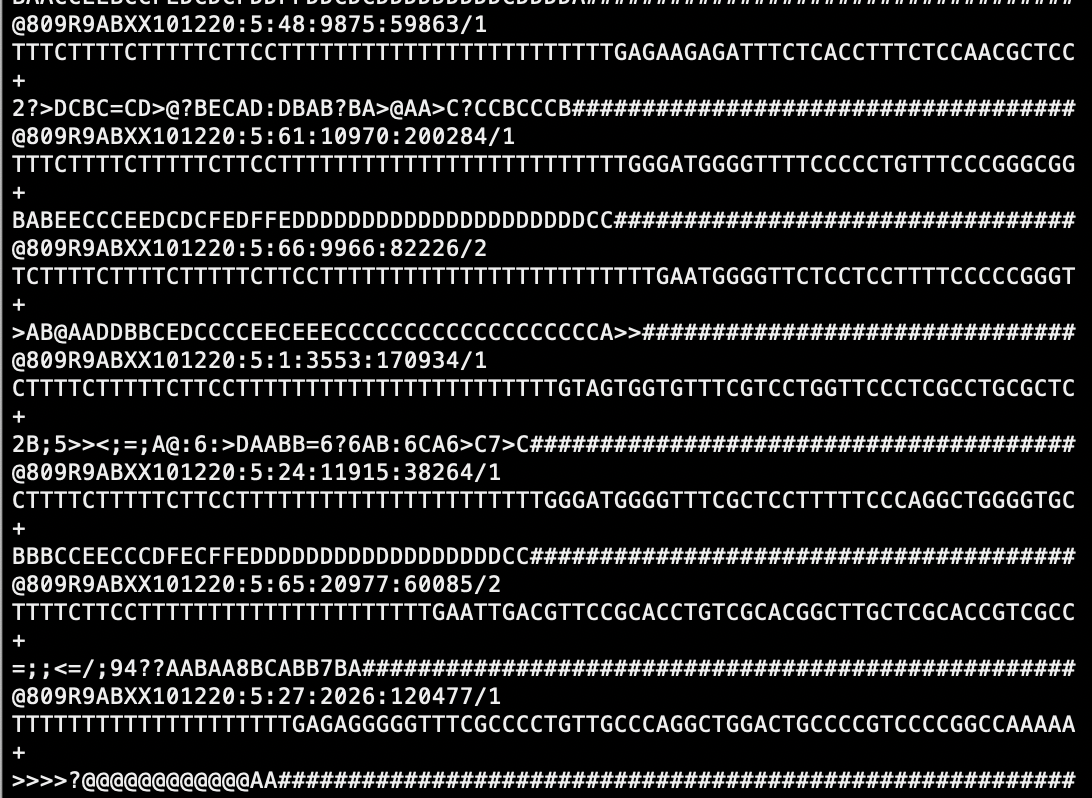
\includegraphics[scale=0.7]{fastq}
    \centering
    \caption {Excerpt from a FASTQ file. /1 and /2 at the end of read ID indicate whether read is first or second in pair.}
    \label{fig:fastq}
\end{figure}

Since FASTQ is a large text file with highly repetitive content it is typically stored in a compressed manner.

\subsubsection{SAM/BAM}

The Sequence Alignment Map (SAM) text file format and its accompanying binary compressed version BAM was created for sequencing data storage and analysis in the context of the 1000 genomes project\autocite{li2009sequence}. These files provide additional fields on top of the ones available in FASTA/FASTQ in order to relay information related to sequence alignment to a reference genome, and are the most widely used format for storing DNA sequencing data today. A SAM file consists of a header and a body. These are described below. All tables, descriptions, and definitions in this section are reproduced or adapted from the SAM file specification at https://samtools.github.io/hts-specs/SAMv1.pdf.

\paragraph{SAM Header}
Each line of the header begins with the character `{\tt @}' followed by a header record (see Table \ref{tab:sam_file_header}). Each line is TAB-delimited and, apart from {\tt @CO} lines,
each data field follows the format `{\tt TAG:VALUE}' where {\tt TAG} is a two-character string that defines the format and content of {\tt VALUE}.

\begin{table}
    \caption{SAM file header record and column definition. Tags listed with `*' are required. (adapted from https://samtools.github.io/hts-specs/SAMv1.pdf)}
    \label{tab:sam_file_header}
\small
\begin{longtable}{|l|l|p{13.5cm}|}
  \cline{1-3}
  \multicolumn{2}{|l|}{\bf Tag} & {\bf Description} \\
  \cline{1-3}
  \multicolumn{2}{|l}{\tt @HD} & The header line. The first line if present. \\\cline{2-3}
  & {\tt VN}* & Format version. \emph{Accepted format}: {\tt /\char94[0-9]+\char92.[0-9]+\$/}.\\\cline{2-3}
  & {\tt SO} & Sorting order of alignments. \emph{Valid values}: {\tt unknown} (default), {\tt
    unsorted}, {\tt queryname} and {\tt coordinate}.\\\cline{2-3}
  & {\tt GO} & Grouping of alignments, indicating that similar alignment records
    are grouped together but the file is not necessarily sorted overall.
    \emph{Valid values}: {\tt none} (default), {\tt query} (alignments are
    grouped by {\sf QNAME}), and {\tt reference} (alignments are grouped by
    {\sf RNAME}/{\sf POS}).\\\cline{1-3}
  & {\tt SS} & Sub-sorting order of alignments. Valid values are of the form \emph{sort-order}{\tt :}\emph{sub-sort}, where \emph{sort-order} is the same value stored in the {\tt SO} tag and \emph{sub-sort} is an implementation-dependent colon-separated string further describing the sort order. 
    \emph{Regular expression}: {\tt (coordinate|queryname|unsorted)(:[\verb"A-Za-z0-9_-"]+)+}\\\cline{1-3}
  \multicolumn{2}{|l}{\tt @SQ} & Reference sequence dictionary. The order of {\tt @SQ} lines defines the alignment sorting order.\\\cline{2-3}
  & {\tt SN}* & Reference sequence name.
The {\tt SN} tags and all individual {\tt AN} names in all {\tt @SQ} lines
must be distinct.
  The value of this field is used in the
  alignment records in {\sf RNAME} and {\sf RNEXT} fields. Regular expression: {\tt [!-)+-\char60\char62-\char126][!-\char126]*}\\\cline{2-3}
  & {\tt LN}* & Reference sequence length. \emph{Range}: $[1,\,2^{31}-1]$\\\cline{2-3}
  & {\tt AH} & Indicates that this sequence is an alternate locus.\\\cline{2-3}
  & {\tt AN} & Alternative reference sequence names.\\\cline{2-3}
  & {\tt AS} & Genome assembly identifier. \\\cline{2-3}
  & {\tt DS} & Description.  UTF-8 encoding may be used.\\\cline{2-3}
  & {\tt M5} & MD5 checksum of the sequence.\\\cline{2-3}
  & {\tt SP} & Species.\\\cline{2-3}
  & {\tt UR} & URI of the sequence.\\\cline{1-3}
  \multicolumn{2}{|l}{\tt @RG} & Read group. Unordered multiple {\tt @RG} lines are allowed.\\\cline{2-3}
  & {\tt ID}* & Read group identifier. Each {\tt @RG} line must have a unique {\tt ID}.\\\cline{2-3}
  & {\tt BC} & Barcode sequence identifying the sample or library.\\\cline{2-3}
  & {\tt CN} & Name of sequencing center producing the read.\\\cline{2-3}
  & {\tt DS} & Description.  UTF-8 encoding may be used.\\\cline{2-3}
  & {\tt DT} & Date the run was produced (ISO8601 date or date/time).\\\cline{2-3}
  & {\tt FO} & Flow order. The array of nucleotide bases that correspond to the nucleotides used for each flow of each read.\\\cline{2-3}
  & {\tt KS} & The array of nucleotide bases that correspond to the key sequence of each read.\\\cline{2-3}
  & {\tt LB} & Library.\\\cline{2-3}
  & {\tt PG} & Programs used for processing the read group.\\\cline{2-3}
  & {\tt PI} & Predicted median insert size.\\\cline{2-3}
  & {\tt PL} & Platform/technology used to produce the reads. \emph{Valid values}:
  {\tt CAPILLARY}, {\tt LS454}, {\tt ILLUMINA}, {\tt SOLID}, {\tt HELICOS}, {\tt IONTORRENT}, {\tt ONT}, and {\tt PACBIO}.\\\cline{2-3}
  & {\tt PM} & Platform model. Free-form text providing further details of the
  platform/technology used.\\\cline{2-3}
  & {\tt PU} & Platform unit (e.g. flowcell-barcode.lane for Illumina or slide for SOLiD). Unique identifier.\\\cline{2-3}
  & {\tt SM} & Sample. Use pool name where a pool is being sequenced.\\\cline{1-3}
  \multicolumn{2}{|l}{\tt @PG} & Program. \\\cline{2-3}
  & {\tt ID}* & Program record identifier. Each {\tt @PG} line must have a unique {\tt ID}.
  	The value of {\tt ID} is used in the alignment {\tt PG} tag and {\tt PP} tags of other {\tt @PG} lines.
	{\tt PG} IDs may be modified when merging SAM files in order to handle collisions.\\\cline{2-3}
  & {\tt PN} & Program name \\\cline{2-3}
  & {\tt CL} & Command line.  UTF-8 encoding may be used. \\\cline{2-3}
  & {\tt PP} & Previous {\tt @PG-ID}. Must match another {\tt @PG} header's {\tt ID} tag.
  	{\tt @PG} records may be chained using {\tt PP} tag, with the last record in the chain
	having no {\tt PP} tag. This chain defines the order of programs that have been applied to the alignment.\\\cline{2-3}
  & {\tt DS} & Description.  UTF-8 encoding may be used.\\\cline{2-3}
  & {\tt VN} & Program version \\\cline{1-3}
  \multicolumn{2}{|l}{\tt @CO} & One-line text comment. Unordered multiple {\tt @CO} lines are allowed. UTF-8 encoding may be used.\\
  \cline{1-3}

\end{longtable}
\end{table}

\paragraph{SAM Body}
The body of a SAM file contains alignment records (see Section \ref{sec:bg_alignment} on details of alignment algorithms). Each record has 11 mandatory fields. These fields always appear in the same order and must be present, but their values may be `0' or `*' (depending on the field) if the corresponding information is unavailable. Table \ref{tab:sam_file_body_mandatory_fields} lists the mandatory fields in the SAM format:
\begin{table}
    \caption{SAM file alignment record mandatory column definition. (adapted from https://samtools.github.io/hts-specs/SAMv1.pdf)}
    \label{tab:sam_file_body_mandatory_fields}
\small
\begin{tabular}{rllll}

  \hline
  {\bf Col} & {\bf Field} & {\bf Type} & {\bf Regexp/Range} & {\bf Brief description} \\
  \hline
  1 & {\sf QNAME} & String & \verb:[!-?A-~]{1,254}: & Query template NAME\\
  2 & {\sf FLAG} & Int & $[0,\,2^{16}-1]$ & bitwise FLAG \\
  3 & {\sf RNAME} & String & {\tt \char92*|[!-()+-\char60\char62-\char126][!-\char126]*} & Reference sequence NAME\\
  4 & {\sf POS} & Int & $[0,\,2^{31}-1]$ & 1-based leftmost mapping POSition \\
  5 & {\sf MAPQ} & Int & $[0,\,2^8-1]$ & MAPping Quality \\
  6 & {\sf CIGAR} & String & {\tt \char92*|([0-9]+[MIDNSHPX=])+} & CIGAR string \\
  7 & {\sf RNEXT} & String & {\tt \char92*|=|[!-()+-\char60\char62-\char126][!-\char126]*} & Ref. name of the mate/next read\\
  8 & {\sf PNEXT} & Int & $[0,\,2^{31}-1]$ & Position of the mate/next read \\
  9 & {\sf TLEN} & Int & $[-2^{31}+1,\,2^{31}-1]$ & observed Template LENgth \\
  10 & {\sf SEQ} & String & {\tt \char92*|[A-Za-z=.]+} & segment SEQuence\\
  11 & {\sf QUAL} & String & {\tt [!-\char126]+} & ASCII of Phred-scaled base QUALity+33 \\
  \hline

\end{tabular}
\end{table}
Alignment records represent the information contained in a sequencing read subsequent to it being aligned to a reference genome (see Figure \ref{fig:read_pair}).

\begin{figure}[H]
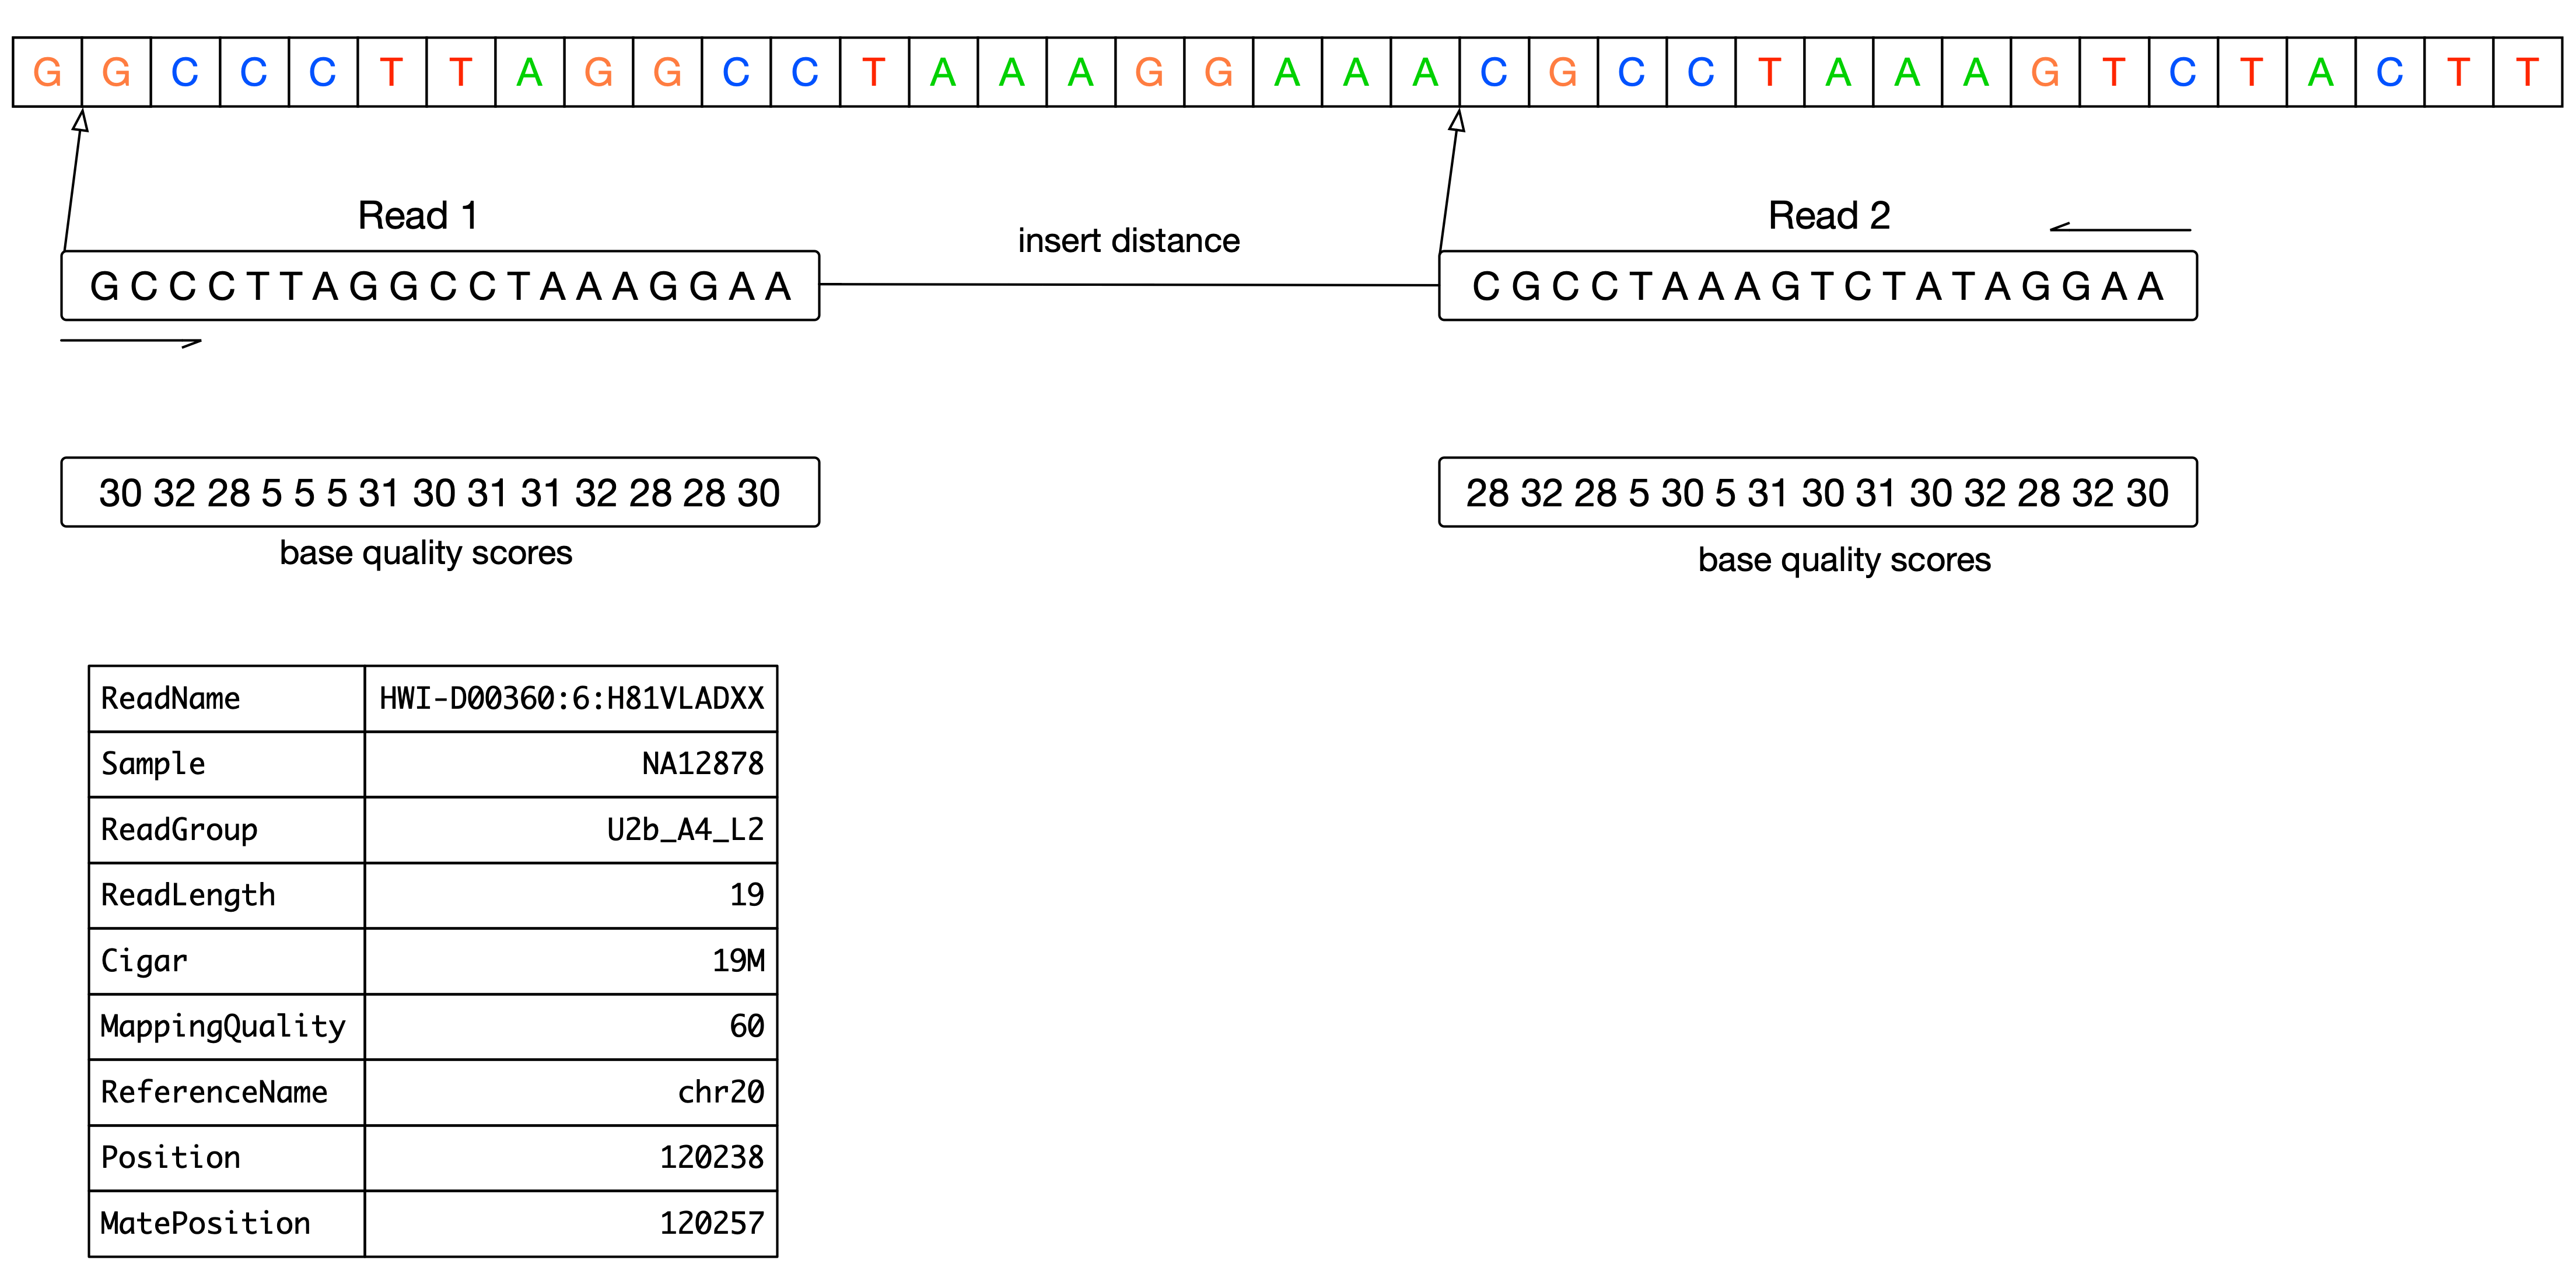
\includegraphics[scale=0.40]{read_pair}
\centering
\caption {A read-pair that is aligned to the reference.}
\label{fig:read_pair}
\end{figure}

\begin{enumerate}
    \item {\sf QNAME}: Query template NAME. Reads/segments having identical {\sf QNAME} are regarded to come from the same template. A {\sf QNAME} `{\tt *}' indicates the information is unavailable.  In a SAM file, a read may occupy
        multiple alignment lines, when its alignment is chimeric or when multiple mappings are given.
    \item {\sf FLAG}: Combination of bitwise FLAGs. Each bit is explained in the following table:
      \begin{center}\small
      \begin{tabular}{rrl}
      \hline
      \multicolumn{2}{c}{Bit} & Description\\
      \hline
        1 &    0x1 & template having multiple segments in sequencing \\
        2 &    0x2 & each segment properly aligned according to the aligner \\
        4 &    0x4 & segment unmapped \\
        8 &    0x8 & next segment in the template unmapped \\
       16 &   0x10 & {\sf SEQ} being reverse complemented \\
       32 &   0x20 & {\sf SEQ} of the next segment in the template being reverse complemented \\
       64 &   0x40 & the first segment in the template \\
      128 &   0x80 & the last segment in the template \\
      256 &  0x100 & secondary alignment \\
      512 &  0x200 & not passing filters, such as platform/vendor quality controls \\
     1024 &  0x400 & PCR or optical duplicate \\
     2048 &  0x800 & supplementary alignment \\
      \hline
      \end{tabular}
      \end{center}
      \begin{itemize}
      \item For each read/contig in a SAM file, it is required that one and only
        one line associated with the read satisfies \mbox{`{\sf FLAG} {\tt \& 0x900
        == 0}'}. This line is called the \emph{primary line} of the read.
      \item Bit 0x100 marks the alignment not to be used in certain analyses
        when the tools in use are aware of this bit. It is typically used to
        flag alternative mappings when multiple mappings are presented in a SAM.
      \item Bit 0x800 indicates that the corresponding alignment line is part of
        a chimeric alignment. A line flagged with 0x800 is called as a \emph{supplementary line}.
      \item Bit 0x4 is the only reliable place to tell whether the read
        is unmapped. If 0x4 is set, no assumptions can be made about {\sf
          RNAME}, {\sf POS}, {\sf CIGAR}, {\sf MAPQ}, and bits 0x2, 0x100,
        and 0x800.
      \item Bit 0x10 indicates whether {\sf SEQ} has been reverse complemented
        and {\sf QUAL} reversed.
        When bit~0x4 is unset, this corresponds to the strand to which the
        segment has been mapped.
        When 0x4 is set, this indicates whether the unmapped read is stored
        in its original orientation as it came off the sequencing machine.
      \item Bits 0x40 and 0x80 reflect the read ordering within each template
        inherent in the sequencing technology used.\footnote{For example,
        in Illumina paired-end sequencing, {\sf first}~(0x40) corresponds to
        the R1~`forward' read and {\sf last}~(0x80) to the R2~`reverse' read.
        (Despite the terminology, this is unrelated to the segments' orientations
        when they are mapped: either, neither, or both may have their
        {\sf reverse} flag bits~(0x10) set after mapping.)}
        If 0x40 and 0x80 are both set, the read is part of a linear
        template, but it is neither the first nor the last read. If both
        0x40 and 0x80 are unset, the index of the read in the template
        is unknown. This may happen for a non-linear template or when this
        information is lost during data processing.
      \item If 0x1 is unset, no assumptions can be made about 0x2, 0x8,
        0x20, 0x40 and 0x80.
      \item Bits that are not listed in the table are reserved for future use.
        They should not be set when writing and should be ignored on reading
        by current software.
      \end{itemize}
    \item {\sf RNAME}: Reference sequence NAME of the alignment. If {\tt
        @SQ} header lines are present, {\sf RNAME} (if not `*') must be
      present in one of the {\tt SQ-SN} tag. An unmapped segment without
      coordinate has a `*' at this field. However, an unmapped segment may
      also have an ordinary coordinate such that it can be placed at a
      desired position after sorting. If {\sf RNAME} is `*', no assumptions
      can be made about {\sf POS} and {\sf CIGAR}.
    \item {\sf POS}: 1-based leftmost mapping POSition of the first {\sf
        CIGAR} operation that ``consumes'' a reference base (see table below).
        The first base in a reference sequence has coordinate 1. {\sf
        POS} is set as 0 for an unmapped read without coordinate. If {\sf
        POS} is 0, no assumptions can be made about {\sf RNAME} and {\sf
        CIGAR}.
    \item {\sf MAPQ}: MAPping Quality. It equals
      $-10\log_{10}\Pr\{\mbox{mapping position is wrong}\}$, rounded to the
      nearest integer. A value 255 indicates that the mapping quality is not
      available.
    \item {\sf CIGAR}: CIGAR string. The CIGAR operations are given in the
      following table (set `*' if unavailable):
      \begin{center}
      \begin{tabular}{cclcc}
      \toprule
      Op & BAM & Description & \makecell{Consumes \\ query} & \makecell{Consumes \\ reference}\\
      \midrule
      {\tt M} & 0 & alignment match (can be a sequence match or mismatch)       & yes & yes \\
      {\tt I} & 1 & insertion to the reference                                  & yes & no  \\
      {\tt D} & 2 & deletion from the reference                                 & no  & yes \\
      {\tt N} & 3 & skipped region from the reference                           & no  & yes \\
      {\tt S} & 4 & soft clipping (clipped sequences present in {\sf SEQ})      & yes & no  \\
      {\tt H} & 5 & hard clipping (clipped sequences NOT present in {\sf SEQ})  & no  & no  \\
      {\tt P} & 6 & padding (silent deletion from padded reference)             & no  & no  \\
      {\tt =} & 7 & sequence match                                              & yes & yes \\
      {\tt X} & 8 & sequence mismatch                                           & yes & yes \\
      \bottomrule
      \end{tabular}
      \end{center}
      \begin{figure}[H]
        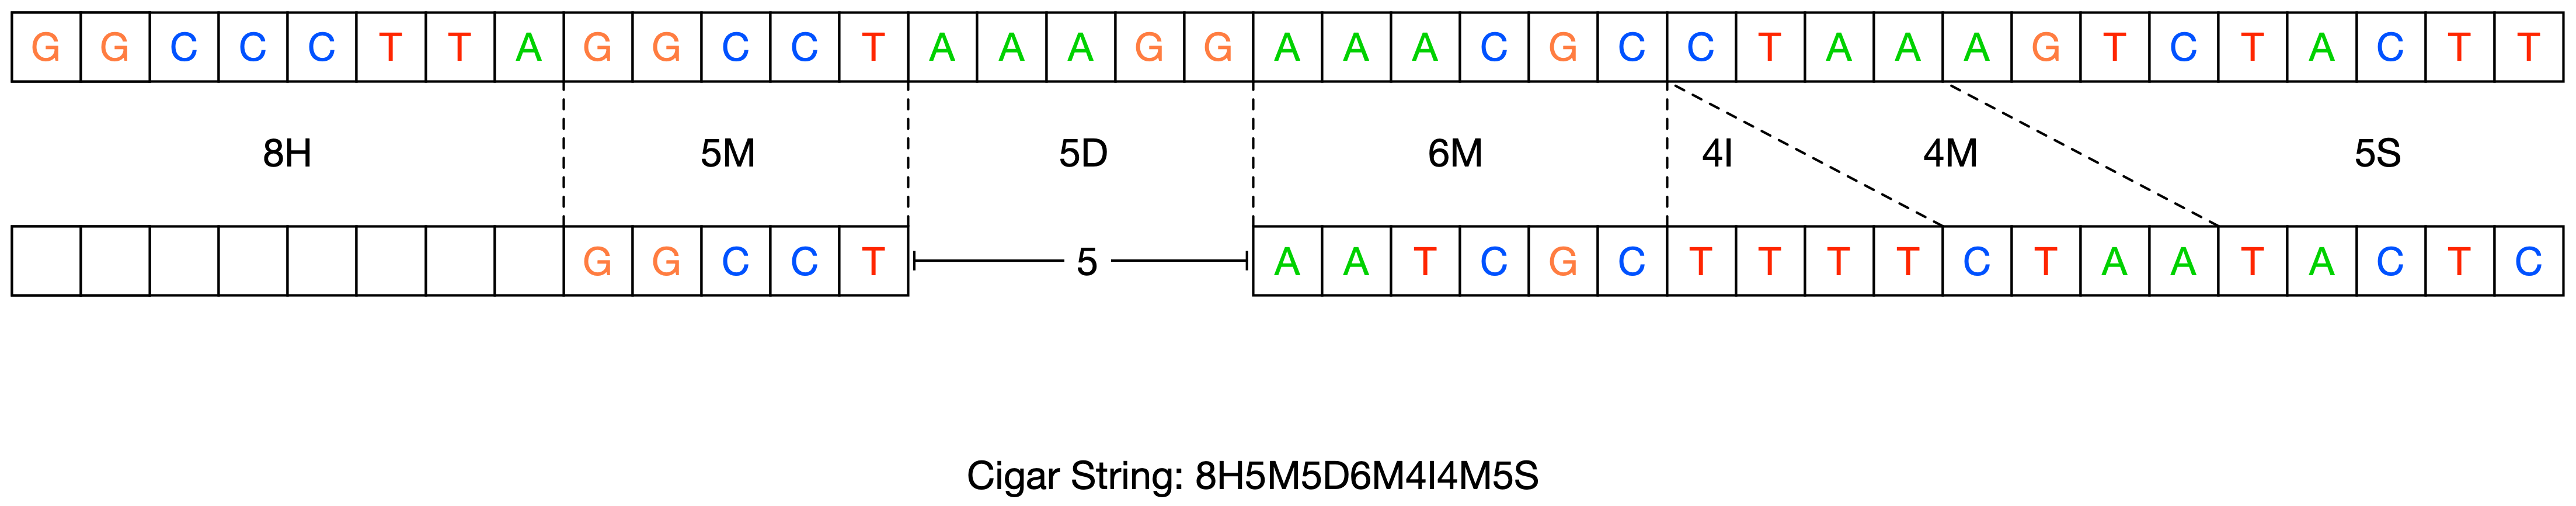
\includegraphics[scale=0.40]{cigar_string}
        \centering
        \caption {Example of an alignment CIGAR string.}
        \label{fig:cigar_string}
        \end{figure}
      \begin{itemize}
      \item ``Consumes query'' and ``consumes reference'' indicate
        whether the CIGAR operation causes the alignment to step along the
        query sequence and the reference sequence respectively.
      \item {\tt H} can only be present as the first and/or last operation.
      \item {\tt S} may only have {\tt H} operations between them and the
        ends of the {\sf CIGAR} string.
      \item For mRNA-to-genome alignment, an {\tt N} operation represents an
        intron. For other types of alignments, the interpretation of {\tt N}
        is not defined.
      \item Sum of lengths of the {\tt M/I/S/=/X} operations shall equal
        the length of {\sf SEQ}.
      \end{itemize}
    \item {\sf RNEXT}: Reference sequence name of the primary alignment of the NEXT read in the
      template. For the last read, the next read is the first
      read in the template. If {\tt @SQ} header lines are present, {\sf
        RNEXT} (if not `*' or `=') must be present in one of the {\tt SQ-SN}
      tag. This field is set as `*' when the information is unavailable, and
      set as `=' if {\sf RNEXT} is identical {\sf RNAME}. If not `=' and the
      next read in the template has one primary mapping (see also bit
      0x100 in {\sf FLAG}), this field is identical to {\sf RNAME} at the primary line of the
      next read.  If {\sf
        RNEXT} is `*', no assumptions can be made on {\sf PNEXT} and bit
      0x20.
    \item {\sf PNEXT}: 1-based Position of the primary alignment of the NEXT read in the template. Set as
      0 when the information is unavailable. This field equals {\sf POS} at the primary line of
      the next read. If {\sf PNEXT} is 0, no assumptions can be made on
      {\sf RNEXT} and bit 0x20.
    \item {\sf TLEN}: signed observed Template LENgth. If all segments are
      mapped to the same reference, the unsigned observed template length
      equals the number of bases from the leftmost mapped base to the
      rightmost mapped base. The leftmost segment has a plus sign and the
      rightmost has a minus sign. The sign of segments in the middle is
      undefined. It is set as 0 for single-segment template or when the
      information is unavailable.
    \item {\sf SEQ}: segment SEQuence. This field can be a `*' when the
      sequence is not stored. If not a `*', the length of the sequence must
      equal the sum of lengths of {\tt M/I/S/=/X} operations in {\sf CIGAR}.
      An `=' denotes the base is identical to the reference base. No
      assumptions can be made on the letter cases.
    \item {\sf QUAL}: ASCII of base QUALity plus 33 (same as the quality
      string in the Sanger FASTQ format). A base quality is the phred-scaled
      base error probability which equals $-10\log_{10}\Pr\{\mbox{base is
        wrong}\}$. This field can be a `*' when quality is not stored. If
      not a `*', {\sf SEQ} must not be a `*' and the length of the quality string
      ought to equal the length of {\sf SEQ}.
    \end{enumerate}
\paragraph{BAM Files}

BAM files are SAM files that have been compressed with block gzip compression\autocite{li2011tabix}. If the reads inside the BAM file are sorted in increasing order of reference coordinate, the BAM file supports random access via a supplementary BAM index (\emph{*.bam.bai}) file. Each block inside a BAM file is a separate gzip archive up to 64Kb in size with extra metadata to encode the read positions contained inside the block. The BAM index file contains offsets into the BAM file that correspond to particular genomic coordinate ranges. The BAM file this provides a binary compressed structure that supports indexed search on genomic coordinates. No other indexing, including by ID, is currently supported. The majority of DNA sequencing data in the world is currently stored as BAM files.

\subsubsection{VCF Files}
The Variant Call Format (VCF)\autocite{danecek2011variant} is a type of text file that was created in the context of the 1000 Genomes project to allow the representation of various types of genetic variation that are discovered via NGS experiments. VCF files describe variants in a refererence-relative manner - i.e. all genetic variation is shown with respect to a given reference genome build. VCF files have a tabular form and allow one to describe genetic variants as they occur in (or are absent from) a entire cohort of samples using a single file. This file format, despite several significant limitations, has become the widely adopted standard for representing genetic variation. All descriptions in this section have been reproduced or adapted from the 2011 Danecek et al. paper and the VCF specification ()   

A VCF file consists of the following sections - Meta-information section describes the format and content of the data contained in the file, header section specifies the columns present in the file, data section contains the actual variant calls that are being described.

\paragraph{Meta-information}
The meta-information section contains a number of lines that describe the data section. The first line of this section is a \emph{fileformat} line that specifies what version of the VCF spec the file adheres to. There can be any number of lines describing INFO fields. These fields are populated into the INFO column of the data section. A single INFO field may describe a single value or a tuple of values. These values can be Integer, Float, Flag, Character, or String. All of the INFO fields thus described are to be placed into the INFO column as a string of semi-colon-separated key-value pairs. The FILTER field describes any filters that have been applied to the variants. The FORMAT field describes the format of the genotype columns that are specified in the data section. The ALT field describes symbolic alternate alleles, that result from variants that have been called but not accurately genotyped. The \emph{contig} field lists the contigs that the variants specified in the file have been called relative to (typically these are chromosome names from the reference sequence). The SAMPLE field specifies the samples that the variants map to. The PEDIGREE field specifies pedigree relationships between samples in the file.

\paragraph{Header}
The header section is a single tab-delimited line that lists what columns are present in the body. The mandatory columns are:
\begin{itemize}
    \item \#CHROM
    \item POS
    \item ID
    \item REF
    \item ALT
    \item QUAL
    \item FILTER
    \item INFO
\end{itemize}

If the VCF file contains genotypes then the INFO column is followed by a FORMAT column, followed by one column for each present sample where each column name is the respective sample ID and all sample IDs are unique within the file.

\paragraph{Data}

The data section of a VCF file contains the actual list of variants and their genotypes in all samples in tabular form where the columns align with the header section. The values are tab-separated. Any missing values are indicated with a '.' (dot). The line contents are as follows:

\begin{description}
    \item [CHROM] - An identifier of the chromosome where the variant resides. The ID of the chromosome should match one of the \emph{contig} entries in the meta-information section. All of the variants that belong to a single CHROM should exist in a single contiguous block of rows in a VCF file.
    \item [POS] - 1-based position of the variant with respect to the reference chromosome specified in CHROM. Variant positions should be sorted numerically in increasing order.
    \item [ID] - A semi-colon separated list of unique identifiers, where they exist. If no identifier exists a missing value should be indicated.
    \item [REF] - the reference bases corresponding to the variant location where each base $b \in \{A,C,G,T,N\}$.
    \item [ALT] - a comma separated list of alternative alleles. The alleles do not have to called in any of the samples. Value can be either a String of $b \in \{A,C,G,T,N,*\}$ or a missing value (when there is no variant).
    \item [QUAL] - the PHRED scale variant quality. When ALT is present QUAL is $-10\log_{10}({no variant})$ and when ALT is missing QUAL is $-10\log_{10}({variant})$. If QUAL is unknown then missing value must be specified.
    \item [FILTER] - encodes the filter status. If the variant passes all QC filters the value should be PASS. Otherwise there should be a semi-colon separated list of codes for filters that have not passed. If FILTER information is not available there should be a missing value.
    \item [INFO] - A list of key-value pairs for the additional fields encoded for each variant as specified in the INFO lines of the metadata section. Keys without corresponding values may be used to indicate group membership. There is a number of frequently used reserved keys (see Table \ref{tab:reserved-info}).
\end{description}
 
\begin{table}[H]
    \centering
    \begin{tabularx}{\textwidth}{ | p{2.5cm} | p{1.5cm} | p{1.5cm} | X | }
    \toprule
    Key		& Number	& Type		& Description \\ 
    \midrule
	AA		& 1		& String	& Ancestral allele \\
	AC		& A		& Integer	& Allele count in genotypes, for each ALT allele, in the same order as listed  \\
	AD		& R		& Integer	& Total read depth for each allele \\
	ADF		& R		& Integer	& Read depth for each allele on the forward strand \\
	ADR		& R		& Integer	& Read depth for each allele on the reverse strand \\
	AF		& A		& Float		& Allele frequency for each ALT allele in the same order as listed (estimated from primary data, not called genotypes) \\
	AN		& 1		& Integer	& Total number of alleles in called genotypes \\
	BQ   		& 1		& Float		& RMS base quality \\
	CIGAR		& A		& String	& Cigar string describing how to align an alternate allele to the reference allele \\
	DB		& 0		& Flag		& dbSNP membership \\
	DP		& 1		& Integer	& Combined depth across samples \\
	END		& 1		& Integer	& End position (for use with symbolic alleles) \\
	H2		& 0		& Flag		& HapMap2 membership \\
	H3		& 0		& Flag		& HapMap3 membership \\
	MQ		& 1		& Float		& RMS mapping quality \\
	MQ0   		& 1		& Integer	& Number of MAPQ == 0 reads \\
	NS		& 1		& Integer	& Number of samples with data \\
	SB		& 4		& Integer	& Strand bias \\
	SOMATIC		& 0		& Flag		& Somatic mutation (for cancer genomics) \\
	VALIDATED	& 0		& Flag		& Validated by follow-up experiment \\
    1000G		& 0		& Flag		& 1000 Genomes membership \\
    \bottomrule
    \end{tabularx}
    \caption{Reserved INFO keys (from https://samtools.github.io/hts-specs/VCFv4.3.pdf).}
    \label{tab:reserved-info}
  \end{table}

If genotype information is present, the exact same definition is used for all samples. The FORMAT field specifies a column seprated list of the data types and their order that are present in the genotype columns. This is followed by one data block for each sample that contains the genotype data as described in the FORMAT column. All keys are optional but missing values should be indicated. There is a number of frequently used and reserved keys (see Table \ref{tab:reserved-genotypes}).

\begin{table}[H]
    \centering
      \begin{tabularx}{\textwidth}{ | p{2.5cm} | p{1.5cm} | p{1.5cm} | X | }
        \toprule
        Field		& Number	& Type		& Description \\ 
        \midrule
        AD		& R		& Integer	& Read depth for each allele \\
        ADF		& R		& Integer	& Read depth for each allele on the forward strand \\
        ADR		& R		& Integer	& Read depth for each allele on the reverse strand \\
        DP		& 1		& Integer	& Read depth \\
        EC		& A		& Integer	& Expected alternate allele counts \\
        FT		& 1		& String	& Filter indicating if this genotype was ``called'' \\
        GL		& G		& Float		& Genotype likelihoods \\
        GP		& G		& Float		& Genotype posterior probabilities \\
        GQ		& 1		& Integer	& Conditional genotype quality \\
        GT		& 1		& String	& Genotype \\
        HQ		& 2		& Integer	& Haplotype quality \\
        MQ		& 1		& Integer	& RMS mapping quality \\
        PL		& G		& Integer	& Phred-scaled genotype likelihoods rounded to the closest integer \\
        PQ		& 1		& Integer	& Phasing quality \\
        PS		& 1		& Integer	& Phase set \\
        \bottomrule
    \end{tabularx}
    \caption{Reserved genotype keys (from https://samtools.github.io/hts-specs/VCFv4.3.pdf).}
    \label{tab:reserved-genotypes}
  \end{table}

The following keys are most important and frequently used:

\begin{itemize}
    \item [GT] - The genotype, encoded as allele values separated by / for unphased genotypes and | for phased genotypes. The values are 0 for reference allele, 1 for first allele listed in ALT, 2 for the second, and so on (for instance 0/1 for heterozygous variant in a diploid sample). When a call cannot be made the missing value is used (for instance ./.).
    \item [GL] - Genotype likelihoods. A comma separated list of $log_{10}$ likelihoods for all possible genotypes given the set of REF and ALT alleles at the locus.
    \item [GP] - Genotype posterior probabilities, in the same order as GL field.
    \item [GQ] - Genotype Quality in PHRED scale. Probability the genotype call is wrong given that the site is variant.
    \item [AD] - Allele Depth. Per-sample read depth for each allele.
    \item [DP] - Read Depth. $\sum_i AD_i$.
\end{itemize}

See Listing \ref{lst:vcf_file} for an example of a VCF file.

\subsubsection{Remarks}

The SAM/BAM and VCF file formats have bencome the de-facto standards for representing sequencing read data and genetic variation respectively. Because of this status most computational tools that exist in this space either consume or produce one of these data-types and the data analysis process is influenced by the file access patterns inherent in these standards. This introduces a number of challenges and limitations that have held back scalability of the existing tools to larger data sets. Specifically:

\begin{itemize}
    \item The focus on files for information storage and retrieval implies that sophisticated file management schemes must be deployed for successful management of large cohorts of samples. This includes concerns of data security, and data migration that must be implemented at the file-system level.
    \item Storage of sequence data at sample level of granularity in SAM/BAM files creates very large files that are typically greater than 150 GB in size per sample and are thus quite cumbersome to work with.
    \item Lack of usage of databases implies only basic indexing and querying schemes are possible for sequencing and variant data. Large amounts of data thus need to be loaded into memory in order to perform basic queries.
    \item Indexing only by genomic coordinate implies a coordinate-based data traversal mechanisms that process a genome linearly from beginning to the end.
    \item The multi-sample VCF format makes it easy to interpret all carriers for a single variant (by reading a single row), but is not well suited for interrogating all variants for a single individual (scanning all rows for a single column) in a text file.
    \item Storage of sequencing data in multiple per-sample files does not take advantage of extreme sequence similarity between samples at a given genomic locus, thus reducing the opportunities for data compression and driving up project costs for large scale sequencing efforts where data set size exceeds 1PB.
\end{itemize}

The stream-based approach adopted by the Rheos framework desribed in this work attempts to address many of the above issues.

\subsection{Base-calling}

\subsection{Alignment}
\label{sec:bg_alignment}


BWA/MEM -
Bowtie - 
Gem - 

\subsection{Raw Data QC}
\label{sec:bg_raw_data_qc}

The data that is generated as part of NGS experiments can have widely varying quality, and may suffer from systematic biases introduced by the experimental protocol employed, the technology used, as well as individual events such as sample contamination\autocites{lauss2013monitoring}{aird2011analyzing}{dohm2008substantial}{cibulskis2011contest}. The effect of low quality data such as sequencing errors on downstream analysis can be quite significant, not only because it may introduce false positive variants in the final output, but also because it can produce a large number of potentially variant sites that need to be evaluated and will consume a large amount additional computational resources to eventually rule out. A wide variety of computational methods exist for examining the data after it has been generated in order to identify and fix or filter out low quality data. The most widely used tools include Picard\autocite{Picard2018toolkit}, FastQC\autocite{andrews2010fastqc}, QC Toolkit\autocite{patel2012ngs}, QC-Chain\autocite{zhou2013qc}, and FASTX-Toolkit\autocite{gordon2010fastx}. These tools evaluate data at two granularities - read-level, and sample-level. Some of these can act on sequencing data pre-alignment, while others either work post-alignment or actively make use of a built-in aligner. The QC process is generally organized into a QC pipeline (see Figure \ref{fig:qc-chain}). Furthermore, some tools, like FastQC and Picard tend to only collect various QC metrics and generate reports, leaving the filtering based on these metrics up to the user, while other tools, such as QC Toolkit and QC-Chain perform the actual filtering themselves.

\begin{figure}[H]
    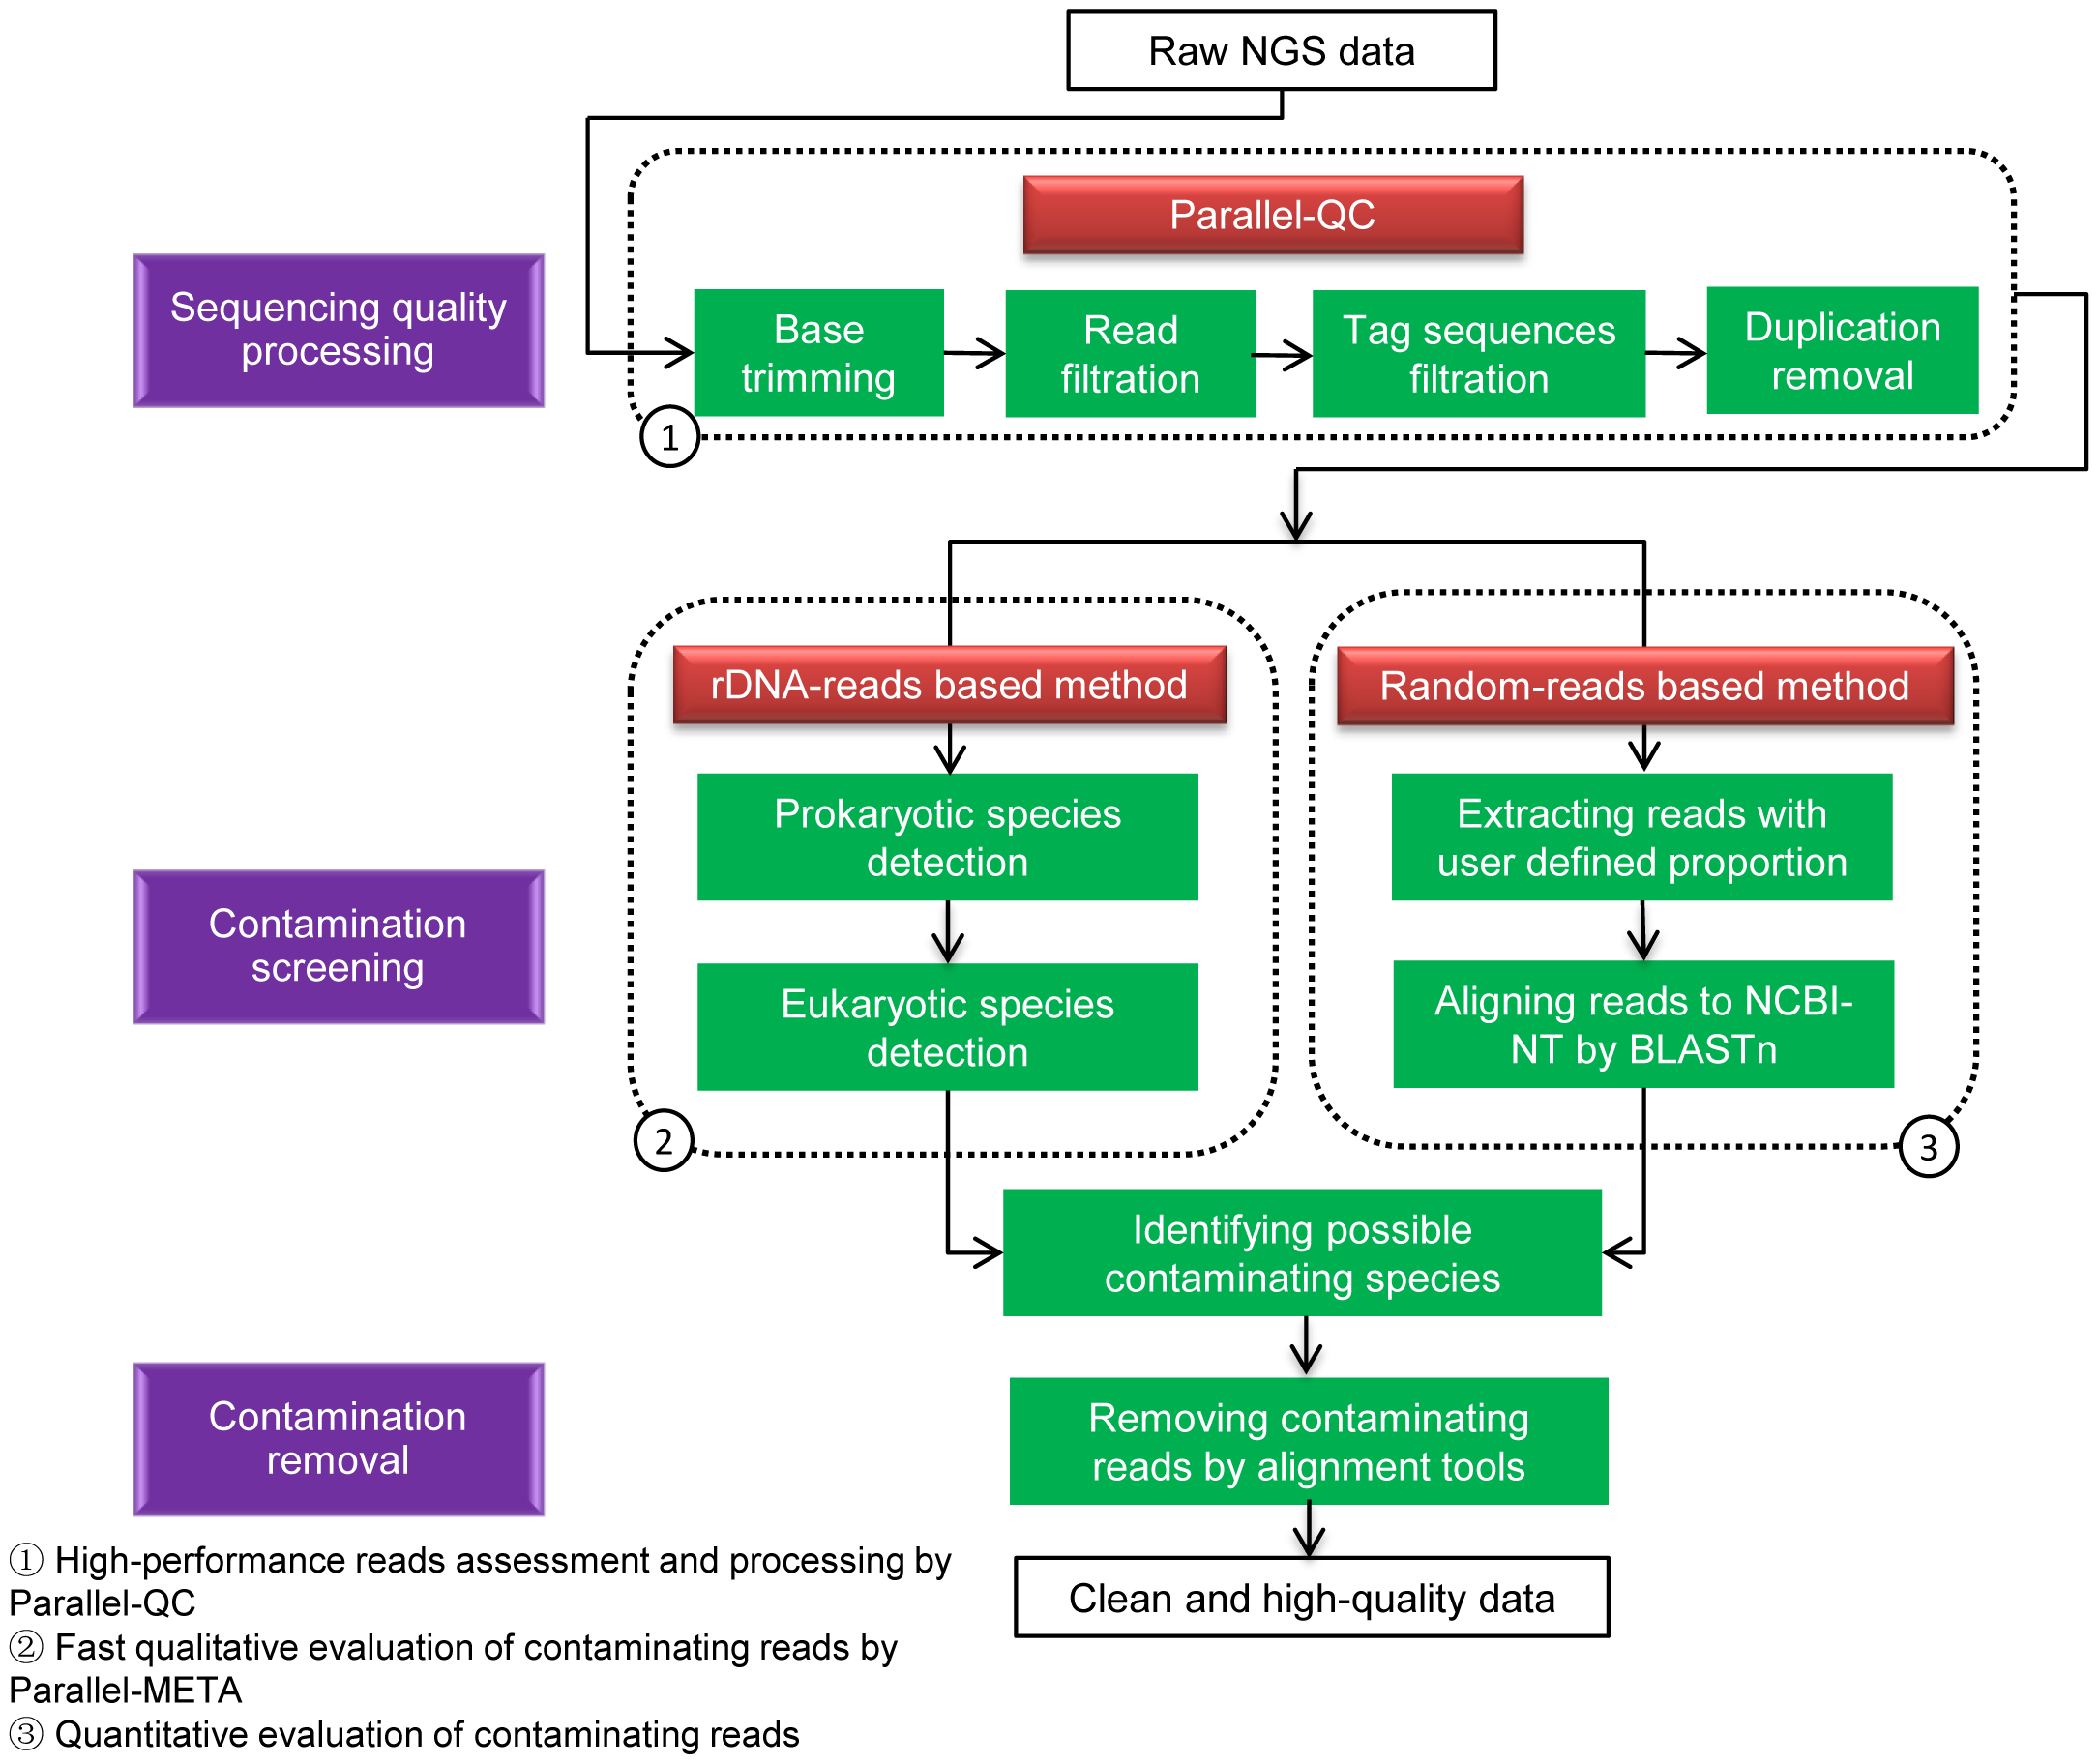
\includegraphics[scale=0.85]{journal.pone.0060234.g001}
    \centering
    \caption {The QC-Chain pipeline involves trimming low quality bases, removal of adapter sequences, removal of duplicate reads, and contamination detection.\autocite{zhou2013qc}.}
    \label{fig:qc-chain}
\end{figure}

At individual read level the following QC measures are of interest:

\begin{description}
    \item [Base Quality Distribution] - Reads in FASTQ format have a base-quality score associated with each nucleotide which serve as estimates of the probability that the base has been called correctly by the base-caller software. Bases towards the end of Illumina reads tend to suffer from deteriorating quality(\autocite{dohm2008substantial} and may not be usable for downstream analysis. 
    \item [Adapter Sequence Presence] - The NGS library preparation protocol involves ligating an adapter sequence to the end of DNA fragments in order to bind the fragment to the sequencing flowcell. Sometimes the sequencing process does not stop at the end of the actual DNA molecule and also sequences the adapter. It is necessary to detect and trim out these adapter sequences as they do not belong to the genome\autocite{bolger2014trimmomatic}.
    \item [Duplicate Detection] - in NGS libraries that use PCR amplification a particular DNA fragment may be sequenced multiple times resulting in increased apparent, and depleted actual coverage of that region of the genome, possibly influencing downstream variant calling efforts. Both Picard\autocite{Picard2018toolkit} and Samtools\autocite{li2011statistical} have utilities for detecting PCR duplicates, although the additional benefit of this processing step may be marginal\autocite{ebbert2016evaluating}.
    \item [Sample Contamination/Sample Swap] - Sample contamination during library preparation may result in the presence of foreign DNA in the generated sequence. The foreign sequence may originate from the same or from foreign species. Furthermore, entire samples may be swapped or mislabelled (for instance, cancer samples with tumour from one patient, but normal sample from another patient). Contamination may be detected by aligning reads to a panel of potentially contaminating species' reference genomes\autocite{zhou2013qc}, or when a surprising number of variants is found in a given genome.
\end{description}

\begin{figure}[H]
    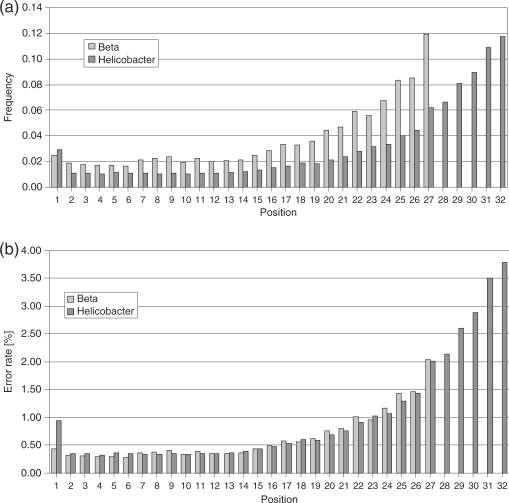
\includegraphics[scale=0.65]{base_errors_read_position}
    \centering
    \caption {Frequency of wrong base calls in Illumina reads based on position in the read from 5' to 3'.\autocite{dohm2008substantial}.}
    \label{fig:base_errors_read_position}
\end{figure}

At the sample level the following QC measures are important:

\begin{description}
    \item [Insert Distribution] - summary statistics (mean, median, standard deviation) related to the distribution of the distance between paired-end reads.
    \item [Per-base Quality Distribution] - distribution of base qualities for each position in a read, aggregated over all reads.
    \begin{figure}[H]
        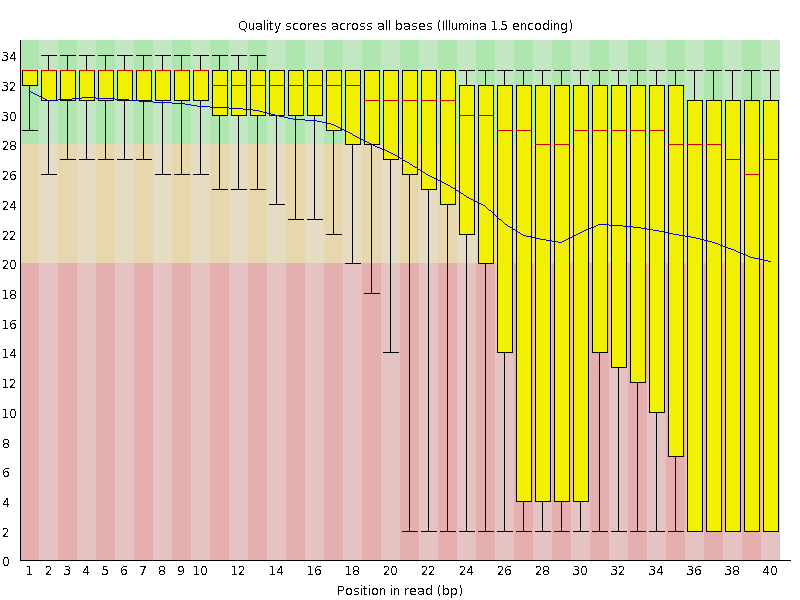
\includegraphics[scale=0.35]{fastqc_per_base_quality}
        \centering
        \caption {from https://www.bioinformatics.babraham.ac.uk/projects/fastqc.}
        \label{fig:fastqc_per_base_quality}
    \end{figure} 
    \item [Per-read Quality Distribution] - distribution of average read qualities.
    \item [Per-base Sequence Content Distribution] - distribution of nucleotide frequencies for each position in a read, aggregated over all reads.
    \begin{figure}[H]
        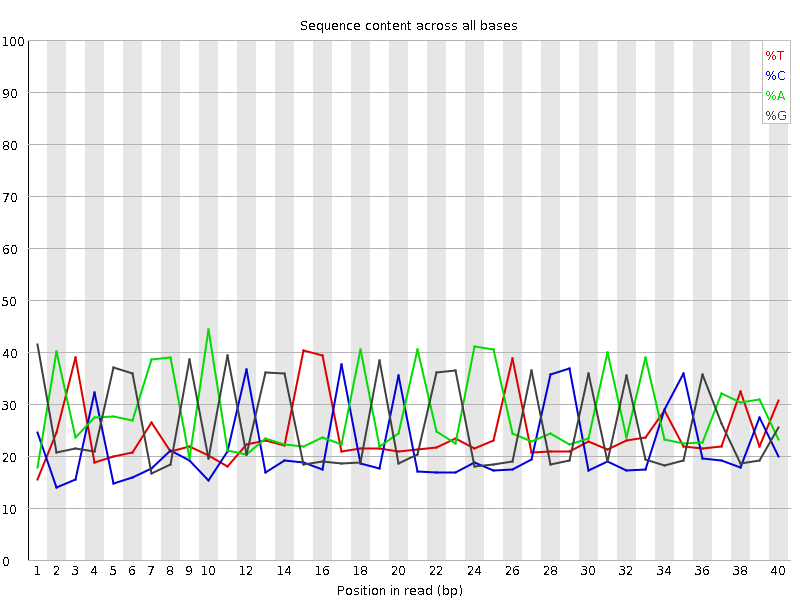
\includegraphics[scale=0.35]{fastqc_sequence_content}
        \centering
        \caption {from https://www.bioinformatics.babraham.ac.uk/projects/fastqc.}
        \label{fig:fastqc_sequence_content}
    \end{figure} 
    \item [Per-read GC Content Distribution] - distribution of average GC content per read.
    \begin{figure}[H]
        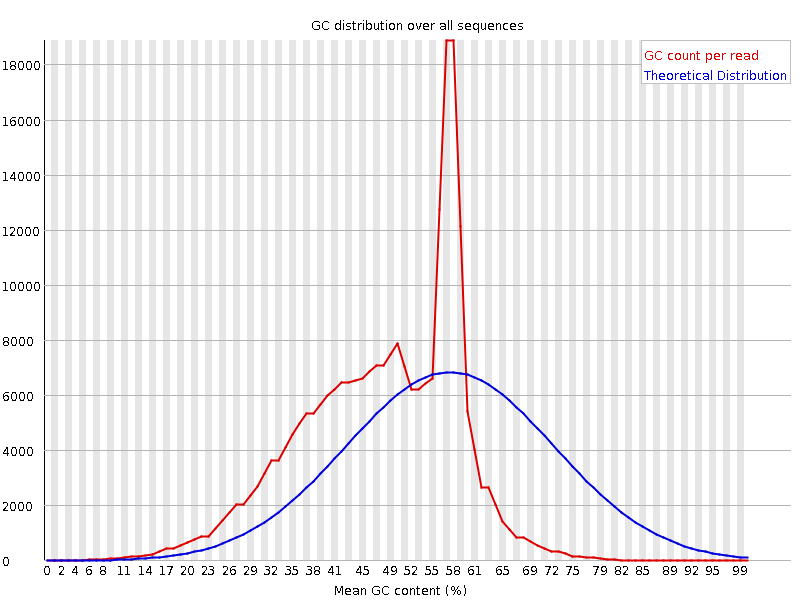
\includegraphics[scale=0.35]{fastqc_gc_content}
        \centering
        \caption {from https://www.bioinformatics.babraham.ac.uk/projects/fastqc.}
        \label{fig:fastqc_gc_content}
    \end{figure}
    
    \item [Read-length Distribution] - summary statistics of read lengths.
    \item [Per-base N Content] - distribution of uncalled bases for each position in a read, aggregated over all reads.
    \item [Sequence Duplication Distribution] - distribution of counts for duplicated sequences.
    \item [Overrepresented Sequence Distribution] - frequency of sequence fragments that occur more frequently that expected.
    \item [Per-base Adapter Content Distribution] - frequency of adapter sequence presence for each position in a read, aggregated over all reads.
    \begin{figure}[H]
        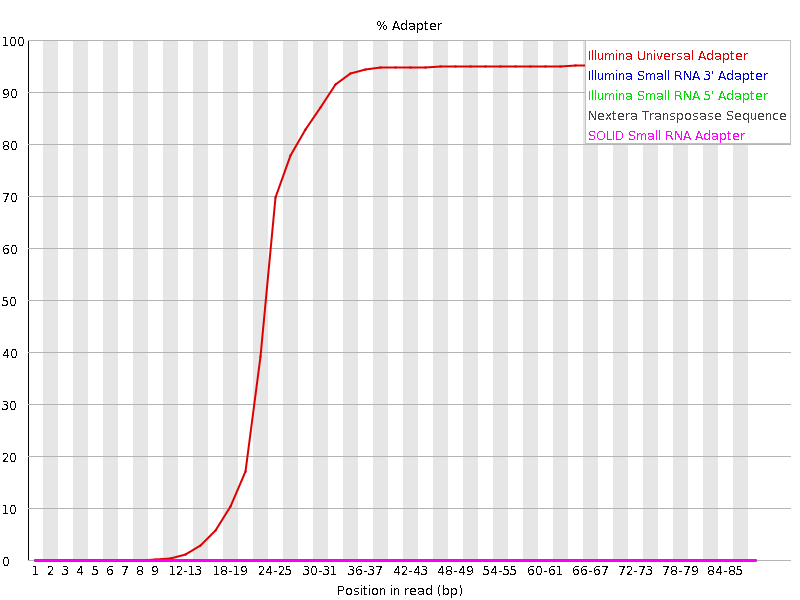
\includegraphics[scale=0.35]{fastqc_adapter_content}
        \centering
        \caption {from https://www.bioinformatics.babraham.ac.uk/projects/fastqc.}
        \label{fig:fastqc_adapter_content}
    \end{figure} 
    
\end{description}

Many other QC metrics can be of interest and are listed on the individual tools' pages (for instance https://broadinstitute.github.io/picard/picard-metric-definitions.html). Once collected, these metrics can be used for visualization, manual curation, threshold-based filtering, or machine learning approaches to QC.

\subsection{Germline SNP Calling}
\label{sec:bg_germline_snp_calling}

Single Nucleotide Polymorphisms or SNPs are locations in an individual's genome where that individual differs from the reference sequence at a single position. The reference sequence is haploid i.e. it provides a single base (for instance T) at every genomic location, whereas the human genome is diploid (there are two copies of each chromosome, and thus two bases at each location) for chromosomes 1-22, and chromosome X for females, while being haploid for chromosomes X and Y for males. Thus, at each genomic location, the human genome may be:

\begin{description}
    \item [Homozygous Reference] - When both alleles carried by the individual at that location match the reference.
    \item [Heterozygous] - When one allele matches the reference and one is different from the reference.
    \item [Homozygous Alternate] - When both alleles are the same and different from the reference.
    \item [Multiallelic] - When both alleles are different from the reference and are different from each other\autocite{hodgkinson2010human}.
\end{description}

SNPs are the most common type of genomic variant, with every individual carrying over 3 million SNPs on average\autocite{shen2013comprehensive}. Furthermore, the presence of certain SNPs is strongly associated with disease\autocite{wellcome2007genome}, where some SNPs are known to be causative\autocite{ingram1957gene}, while others, are merely associated with a disease phenotype\autocite{satake2009genome}. A large number of scientific studies\autocite{hirschhorn2005genome} and clinical practice\autocite{yang2013clinical} is thus enabled by efficient and comprehensive characterization of the gamut of human SNPs to assess their contribution to disease risk, see Figure \ref{fig:genetic_architecture_of_cancer_risk}.

\begin{figure}[H]
    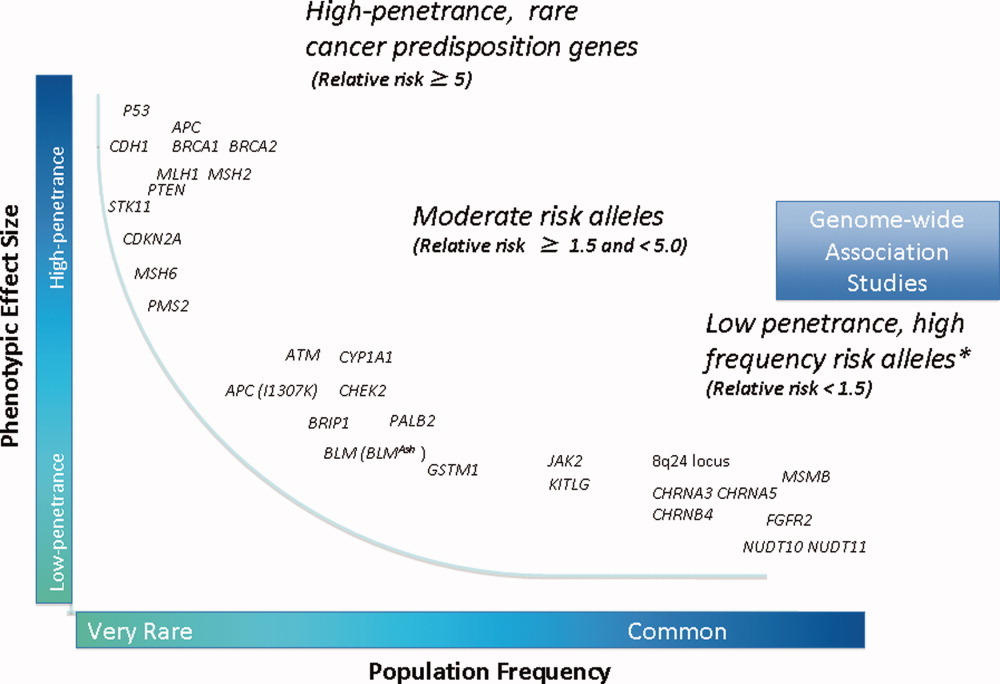
\includegraphics[scale=0.55]{genetic_architecture_of_cancer_risk}
    \centering
    \caption {Distribution of mutations by population frequency against phenotypic effect size.\autocite{weitzel2011genetics}.}
    \label{fig:genetic_architecture_of_cancer_risk}
\end{figure}

There are a number of methods that have been used for assessing SNPs with the aid of microarry technology\autocite{heller2002dna}, but here we focus on methods that make use of Next Generation Sequencing (NGS). Since the primary data type generated by NGS is a sequencing read, most presently used methods for SNP detection rely on investigating the collection of sequencing reads that overlap each genomic locus and comparing the observed data to the reference sequence. It is important to distinguish two typically separate activities that take place as part of SNP calling - variant calling, and genotyping. Variant calling attempts to locate positions in the sample genome where that sample is different from the reference, whereas genotyping attempts to assign an actual genotype (e.g. homozygous-alternate), along with a measure of confidence, to each putative variant. We present several of the key computational methods currently used in SNP calling with additional detail. These are:

\begin{itemize}
    \item samtools
    \item freebayes
    \item GATK
    \item platypus
\end{itemize}

These tools have been selected because they have been developed independently, at different institutions, and have been repeatedly demonstrated to produce consistent and high-quality results. See Figure \ref{fig:fb_hc_st_pt} for a recent comparison.

\begin{figure}[H]
    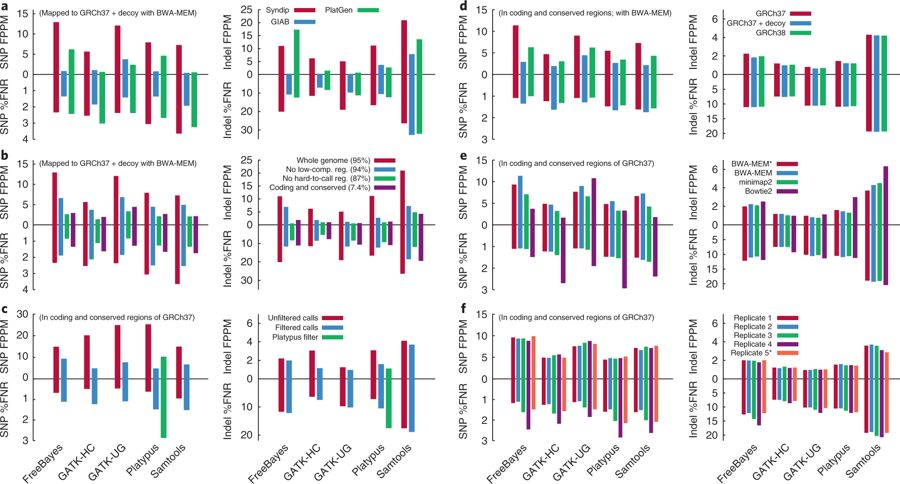
\includegraphics[scale=0.45]{fb_hc_st_pt}
    \centering
    \caption {Comparison of samtools,freebayes, GATK, and platypus on three benchmark data sets - Syndip, GIAB, and PlatGen. Here FPPM - number of false positives per megabase of sequence, and FNR - false negative rate = 100xFN/(TP+FN).\autocite{li2018synthetic}.}
    \label{fig:fb_hc_st_pt}
\end{figure}

\subsubsection{samtools}
Samtools\autocite{li2009sequence} is a software package for genomic data processing developed by Heng Li et al. in the context of the 1000 Genomes Project\autocite{10002010map} and implemented as a C program with a CLI interface. This tool has enjoyed continued and widespread use in the bioinformatics community for the purposes of small variant calling (including SNPs). All of the mathematical results in this section are reproduced from the 2011 paper by Li\autocite{li2011statistical} that describes the method, as well as a set of mathematical notes made available separately by Li\autocite{li2010mathematical} in 2010.

Although the samtools framework could be extended to support calling multi-allelic sites, the framework, as-published, has been developed for calling only bi-allelic variants. Table \ref{tab:samtools_notation} contains commonly used definitions.

\begin{table}[!htb]
    \caption{Samtools common definitions}
    \label{tab:samtools_notation}
    {\begin{tabular}{lp{7cm}}
    \toprule
    Symbol & Description \\
    \midrule
    $n$ & Number of samples \\
    $m_i$ & Ploidy of the $i$-th sample ($1\le i\le n$)\\
    $M$ & Total number of chromosomes in samples: $M=\sum_i m_i$\\
    $d_i$ & Sequencing data (bases and qualities) for the $i$-th sample\\
    $g_i$ & Genotype (the number of reference alleles) of the $i$-th sample \mbox{($0\le g_i\le m_i$)}$^1$\\
    $\phi_k$ & Probability of observing $k$ reference alleles ($\sum_{k=0}^M\phi_k=1$) \\
    $P(A)$ & Probability of an event $A$\\
    $\mathcal{L}_i(\theta)$ & Likelihood function for the $i$-th sample: $\mathcal{L}_i(\theta)=P(d_i|\theta)$ \\
    \bottomrule
    \end{tabular}}
\end{table}

It is additionally assumed that there are $n$ individuals being sequenced with the $i$-th individual having ploidy $m_i$ (typically 2 in practice). At a particular genomic locus, the sequence read data for the $i$-th individual is $d_i$ and the genotype is $g_i$, an integer in $[0,m_i]$, counting the number of reference alleles in the individual at that locus. Furthermore, it is assumed for simplicity that data at individual genomic loci are independent (which isn't necessarily true), as are sequencing and mapping errors between loci and individuals.

Because of the above independence assumptions the joint likelihood function of the data observed for all individuals factors as a product of individual likelihood functions:

\begin{equation}
    \mathcal{L}(\theta)=\prod_{i=1}^n\mathcal{L}_i(\theta)
\end{equation}

Suppose that a single sample $i$ represents an individual of ploidy $m_i$ and a given locus is covered by $k$ reads. The sequencing data $d_i$ is composed of an array of bases where each element has value 1 representing the reference allele and is 0 otherwise. 

\[
d_i=(b_1,\dots,b_k)=(\underbrace{1,\ldots,1}_l,\underbrace{0,\ldots,0}_{k-l})
\]


The error probability of the $j$-th base is $\epsilon_j$, which is taken to be the larger between sequencing and mapping errors for that read. Under the independence assumptions above:

\begin{equation}
    \mathcal{L}_i(0) = P(d_i|0)=\prod_{j=1}^l\epsilon_j\prod_{j=l+1}^k(1-\epsilon_j)=\left(1-\sum_{j=l+1}^k\epsilon_j+o(\epsilon^2)\right)\prod_{j=1}^l\epsilon_j
\end{equation}
\begin{equation}
    \mathcal{L}_i(m_i) = P(d_i|m_i)=\left(1-\sum_{j=1}^l\epsilon_j+o(\epsilon^2)\right)\prod_{j=l+1}^k\epsilon_j
\end{equation}
For $0<g_i<m_i$:
\begin{eqnarray*}\label{eq:gd}
    \mathcal{L}_i(g_i) = P(d_i|g_i)&=&\sum_{a_1=0}^1\cdots\sum_{a_k=0}^1\Pr\{d_i|B_1=a_1,\ldots,B_k=a_k\}\Pr\{B_1=a_1,\ldots,B_k=a_k|g\}\\\nonumber
    &=&\sum_{\vec{a}}\left(\frac{g}{m}\right)^{\sum_j a_j}\left(1-\frac{g}{m}\right)^{k-\sum_j a_j}\cdot\prod_j p_j(a_j)\\\nonumber
    &=&\left(1-\frac{g}{m}\right)^k\prod_j\sum_{a=0}^1 p_j(a)\left(\frac{g}{m-g}\right)^a\\\nonumber
    &=&\left(1-\frac{g}{m}\right)^k\prod_{j=1}^l\left(\epsilon_j+\frac{g}{m-g}(1-\epsilon_j)\right)\prod_{j=l+1}^k\left(1-\epsilon_j+\frac{\epsilon_jg}{m-g}\right)\\\nonumber
    &=&\left(1-\frac{g}{m}\right)^k\left\{\left(\frac{g}{m-g}\right)^l+\left(1-\frac{g}{m-g}\right)\left(\sum_{j=1}^l\epsilon_j-\sum_{j=l+1}^k\epsilon_j\right)+o(\epsilon^2)\right\}
\end{eqnarray*}
where $a=\sum_j a_j$ and
$$
    p_j(a)=\left\{\begin{array}{ll}
    \epsilon_j & \mbox{$a=1$}\\
    1-\epsilon_j & \mbox{$a=0$}\\
    \end{array}\right.
$$

In particular, for a diploid sample ($m=2$), the likelihoods for $g=0,1,2$ are
\begin{eqnarray}
    \label{samtools_diploid_genotype_likelihoods}
    \mathcal{L}(0)&=&\prod_{j=1}^l\epsilon_j\prod_{j=l+1}^k(1-\epsilon_j)\\
    \mathcal{L}(1)&=&\frac{1}{2^k}\\
    \mathcal{L}(2)&=&\prod_{j=1}^l(1-\epsilon_j)\prod_{j=l+1}^k\epsilon_j
\end{eqnarray}

For instance, taking $g_i = 2$ (i.e. the true genotype is homozygous-reference) as an example, and under above independence assumptions, the likelihood of observing the data $d_i$ is the likelihood of sampling $l$ reads without error (the reads match the reference) and $k-l$ reads with error (the reads do not match the reference).

Let $\Phi = \{\phi_k\}$ for $k \in [0,m_i]$ be a prior distribution of genotype probabilities (a model from population genetics, such as Wright-Fisher, can be used, or an empirical distribution from antoher study), the actual genotype for individual $i$ at the given locus is estimated via Bayes' Rule as:

\begin{equation}
    \label{eq:samtools_genotype}
    \hat{g}_i=\argmax_{g_i} \Pr\{G_i=g_i|d_i,\Phi\}=\argmax_{g_i}\frac{P(d_i|g_i)\phi_k}{\sum_{h_i}P(d_i|h_i)\phi_h}=\argmax_{g_i}\frac{\mathcal{L}(g_i)\phi_k}{\sum_{h_i}\mathcal{L}(h_i)\phi_h}
\end{equation}

The variant quality is defined as:

\begin{equation}
    \label{eq:samtools_variant_quality}
    Q_{\rm var}=-10\log_{10}\Pr\{G=m_i|d_i,\Phi\}
\end{equation}

i.e. the Phred-scaled probability that the locus is homozygous reference given the observed data. The locus is called \emph{variant} if the variant quality exceeds a certain pre-defined threshold.

Equations \ref{eq:samtools_genotype} and \ref{eq:samtools_variant_quality} thus represent the key computations corresponding to the activities of SNP genotyping and variant calling that are performed by samtools for each genomic locus in a sample.

\subsubsection{freebayes}

freebayes\autocite{garrison2012haplotype} is a C software package implemented by E. Garrison for discovery and genotyping of SNPs, indels, and other small variants that builds on a previous method by G. Marth\autocite{marth1999general}. Where small means that the variant length is smaller than the size of a sequencing read. Unlike samtools, which looks at all genomic loci independently, freebayes uses local sequence context to guide detection and genotyping of variants, additionally freebayes builds variant haplotypes\autocite{daly2001high} i.e. groups of variants that are inherited together on the same DNA molecule. All of the figures and methematical formuls in this section are reproduced from the 2012 preprint by Garrison et al\autocite{garrison2012haplotype}.

\begin{table}[!htb]
    \caption{Freebayes common definitions}
    \label{tab:freebayes_notation}
    {\begin{tabular}{lp{7cm}}
    \toprule
    Symbol & Description \\
    \midrule
    $n$ & Number of samples \\
    $m_i$ & Copy number of the $i$-th sample ($1\le i\le n$)\\
    $M$ & Total number of copies of each locus in all samples: $M=\sum_i m_i$\\
    $\{b_j: j \in [1,K]\}$ & Set of $K$ distinct alleles present among $M$ copies\\
    $\{C_j: j \in [1,K]\}$ & Corresponding set of allele counts for each $b_K$\\
    $\{f_j: j \in [1,K]\}$ & Corresponding set of allele frequencies for each $b_K$\\
    $G_i$ & Unphased genotype of individual $i$\\
    $\{b_{i_{j}}: i \in [1,n], j \in [1,k_i]\}$ & Set of $k_i$ distinct alleles of $G_i$\\
    $\{c_{i_{j}}: i \in [1,n], j \in [1,k_i]\}$ & Set of $k_i$ allele counts for each $b_{i_{j}}$\\
    $\{f_{i_{j}}: i \in [1,n], j \in [1,k_i], f_i = c_i/k_i\}$ & Set of allele frequencies of $G_i$\\
    $B_i:|B_i| = m_i$ & Multiset of alleles equivalent to $G_i$\\
    $R_i = \{r_j: j \in [1,s_i]\} $ & Set of $s_i$ sequencing observations for each sample $i$ s.t. there are $\sum_{i=1}^n |R_i|$ reads at a given locus\\
    $\{q_j : j \in [1,s_i]\}$ & Mapping quality, i.e. probability that read $r_j$ is mis-mapped against the reference\\
    \bottomrule
    \end{tabular}}
\end{table}

For a set of $n$ individuals the conditional probability of a combination of genotypes given the observed data is assessed simultaneously as:

\begin{equation}
P(G_1,\ldots,G_n|R_1,\ldots,R_n) 
= { P(G_1,\ldots,G_n) P(R_1,\ldots,R_n|G_1,\ldots,G_n) \over P(R_1,\ldots,R_n)} \\
\end{equation}

\begin{equation}
\label{eq:freebayes_main_model}
P(G_1,\ldots,G_n|R_1,\ldots,R_n) = { P(G_1,\ldots,G_n) \prod_{i=1}^n P(R_i|G_i) \over 
\sum_{\forall{G_1,\ldots,G_n}}  P(G_1,\ldots,G_n) \prod_{i=1}^n P(R_i|G_i) }
\end{equation}
    
For a single sample at a particular locus there are $R_i$ reads, and $k_i$ observed alleles - $B'_i = b'_1,\ldots,b'_{k_i}$, which correspond to $b_1,\ldots,b_i$ underlying alleles represented at the given locus. For each observed allele $b'_i$ there is a corresponding count of observations $o_f$ s.t. $: \sum_{j=1}^{k_i} o_j = s_i$ and each $b'_i$ corresponds to a true allele $b_i$. The probability of a single observation $b'_i$ given a genotype in a single sample is:

\begin{equation}
P(b'_i|G) = \sum_{\forall(b_i \in G)} { f_i P(b'_i|b_i) }
\end{equation}

where $f_i$ is the allele frequency of $b_i$ in $G$. The authors introduce the following approximation:


\begin{equation}
P(b'|b) = 
\left\{
        \begin{array}{ll}
                1 & \mbox{if } b' = b \\
                P(error) & \mbox{if } b' \neq b
        \end{array}
\right.
\end{equation}

where $P(error)$ is derived from the base quality score from the sequencing read. Using the above approximation the probability of observing the data $R_i$ given the genotype is estimated as:

\begin{equation}
P(R_i|G) \approx {s_i \choose o_1,\ldots,o_{k_i} } 
\prod_{j=1}^{k_i} { f_{i_j}^{o_j} }
\prod_{l=1}^{s_i} { P(b'_l | b_l) }
\end{equation}

In order to evaluate the posterior probability of a particular combination of genotypes given the data, the authors derive:

\begin{equation}
\label{eq:freebayes_unphasedsampling}
P(G_1,\ldots,G_n | f_1,\ldots,f_k) =
{ M \choose c_1,\ldots,c_k }^{-1}
\prod_{i=1}^n { m_i \choose c_{i_1}, \ldots, c_{i_{k_i}}}
\end{equation}
    
counting the number of ways of selecting a set of unphased genotypes $G_i$ given the allele frequency spectrum $f_k$, and

\begin{equation}
    \label{eq:freebayes_afs}
P(f_1,\ldots,f_k) =
P(a_1,\ldots,a_M) = 
{M! \over \theta \prod_{z=1}^{M-1}(\theta+z)}
\prod_{j=1}^M{\theta^{a_j} \over j^{a_j} a_j!}
\end{equation}

using Ewens' sampling formula\autocite{ewens1972sampling}, where $\theta$ is the population mutation rate and allele frequencies $f_i$ are transformed to frequency counts $a_1,\ldots,a_M : \sum_{c=1}^M{ca_c} = M$ where each $a_f$ is the number of alleles in $b_1,\ldots,b_k$ whose allele count in the sample set is $c$.

Once variants are initially detected using Equation \ref{eq:freebayes_main_model}, the method continues to build local haplotypes grouping variants that are inherited together in dynamically-sized windows based on a distance threshold between successive variants. Each group of variants is combined into a haplotype observation $H_i$, with an assigned quality score that is the minimum of the supporting reads' mapping quality and the minimum base quality of the variant allele observations (bases that span the variants). The size of the window is determined via an iterative process where an initial variant is used as the seed, and all of the reads that overlap it are added. If these reads overlap any other variants, then these are added, along with any reads that overlap them, and so on, until no new variants can be added.

Once the window is determined, the method uses a gradient descent algorithm to find a MAP estimate of the genotype for each sample. It starts with the maximum likelihood estimate for each sample's genotype given the observed data, and then attempts to find a genotype assignment that has a higher posteriror probability across all samples.

\subsubsection{GATK}
The GATK\autocite{depristo2011framework} is not actually a tool that's built solely for SNP calling, but is instead a comprehensive framework for genomic data analysis that includes tools for data pre-processing and QA, SNP and indel calling, CNV calling, and SV calling, as well as post-processing and filtering. It is implemented as a Java program and the latest version makes use of the in-memory computing engine Apache Spark for efficient computation over large data sets. Here we focus on the SNP calling aspects of the framework. There are two components in the GATK that deal with SNP calling, the UnifiedGenotyper, and the HaplotypeCaller. The UnifiedGenotyper is an older component that has been superceded by the HaplotypeCaller for all practical purposes and we focus our attention on it. All of the mathematical formulas and figures, as well as some of the descriptions, in this section have been reproduced from the 2010 manuscript by McKenna et al.\autocite{mckenna2010genome}, the 2011 manuscript by DePristo et al.\autocite{depristo2011framework}, and the GATK website\autocite{gatkwebsite}

\begin{figure}[!htb]
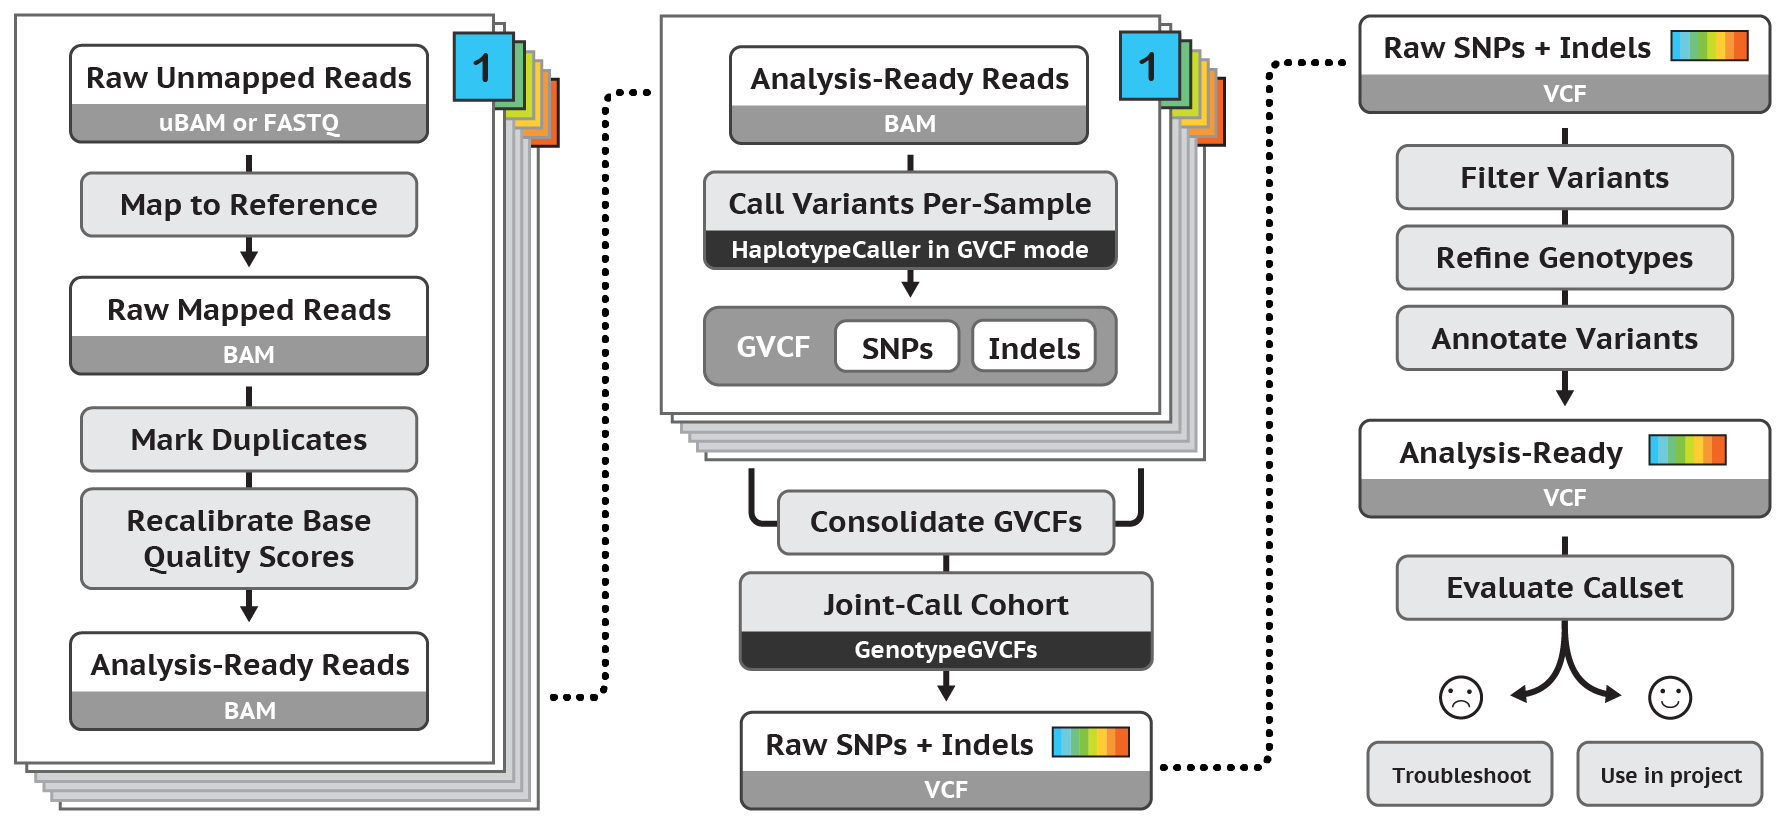
\includegraphics[scale=0.22]{gatk_best_practices}
\centering
\caption {GATK Best Practices pipeline\autocite{gatkwebsite}}
\label{fig:gatk_best_practices}
\end{figure}

The GATK Best Practices pipeline (see Figure \ref{fig:gatk_best_practices}) is a set of best practices published by The Broad Institute that describe how to best use their software. In the context of this section we are primarily interested in the processes that occur in the middle panel of this figure that deal with processing aligned reads to call and genotype variants that will then be used for post-processing and filtering.

The HaplotypeCaller which is the tool that is primarily used for SNP calling takes a continued refinement approach, where the data is processed in the following sequential steps:

\begin{description}
    \item [Define active regions] - The program determines which regions of the genome it needs to operate on (active regions), based on the presence of evidence for variation. 
    \item [Determine haplotypes by assembly of the active region] - For each active region, the program builds a De Bruijn-like graph to reassemble the active region and identifies what are the possible haplotypes present in the data. The program then realigns each haplotype against the reference haplotype using the Smith-Waterman algorithm in order to identify potentially variant sites.
    \item [Determine likelihoods of the haplotypes given the read data] - For each active region, the program performs a pairwise alignment of each read against each haplotype using the PairHMM algorithm. This produces a matrix of likelihoods of haplotypes given the read data. These likelihoods are then marginalized to obtain the likelihoods of alleles for each potentially variant site given the read data.
    \item [Assign sample genotypes] - For each potentially variant site, the program applies Bayes' rule, using the likelihoods of alleles given the read data to calculate the likelihoods of each genotype per sample given the read data observed for that sample. The most likely genotype is then assigned to the sample.
\end{description}

Active regions are defined by targeting loci with high quality reads that are different from the refernce and surrounded by soft-clipped bases (bases in the read that couldn't be aligned by the alignment algorithm). The region is then smoothed by a Gaussian kernel and passed onto variant calling if its profile score exceeds a pre-defined threshold. 

For each active region the GATK performs local assembly by first building a de-Bruijn graph\autocite{compeau2011apply} using just the reference sequence for the active region. The graph is enhanced by comparing each read from the active region and creating nodes in the graph where the read differs from the graph. Edge weights between pairs of nodes are increased when a read passes through that edge. The resulting graph must meet complexity requirements based on the ratio of non-unique to unique kmers and presence of cycles (that are a sign of repetitive sequence). When the graph does not meet complexity requirements it is automatically rebuilt with successively increased kmer sizes. If a sufficiently complex graph cannot be built, the region is discarded because the method is not able to produce a high quality variant call in this case. Once the graph is built it is refined by pruning out paths that are not supported by a sufficient number of reads. By traversing the paths in the graph and selecting those with a high aggregate weight the algorithm builds a list of possible local haplotypes within the active region. Each candidate haplotype is then re-aligned to the reference sequence using Smith-Waterman\autocite{smith1981comparison} alignment to produce a list of potential variant sites that includes SNPs and other potential variants.

Reads from the active region are aligned to each haplotype using a Hidden Markov Model via the PairHMM algorithm\autocite{durbin1998biological} to produce a likelihood of each read given a haplotype. The set of haplotype likelihoods is transformed to a set of likelihoods per allele where for each allele at a given site the the highest scoring likelihood for a given read and a given haplotype that supports that allele is selected. Under a read independence assumption the total likelihood of the allele is computed as the product of read likelihoods.

For each variant locus the probability of each genotype is calculated using:

\begin{equation}
    \label{eq:gatk_genotyping}
P(G|D) = {P(G)P(D|G)\over\sum_i P(G_i)P(D|G_i)}
\end{equation}

where $D$ is the set of reads, $G_i$ is the set of possible genotypes, and under the assumptions of a diploid sample, independent read observations, and independent errors. The prior probability of genotypes $P(G)$ is assumed to be uniform. 

Based on the diploid and independence assumptions:

\begin{equation}
    P(D|G) = \prod_j{\bigg({P(D_j|H_1)\over 2} + {P(Dj|H_2)\over 2}\bigg)}
\end{equation}

where $P(D_j|H_n)$ is the likelihood of read given the haplotype perviously obtained.

The genotype with the highest $P(G|D)$ is emitted as the genotype for that variant.

\subsubsection{Platypus}
Platypus\autocite{rimmer2014integrating} is a Python and C package by Rimmer et al., that provides SNP, indel, and other small and medium (upt to ~1kb) variant calling capabilities utilizing a Bayesian statistical framework built on top of reference-free local assembly of haplotypes. All of the figures and methematical formuls in this section are reproduced from the 2014 Nature Genetics manuscript by Rimmer et al. See Figure \ref{fig:platypus_main_flow} for the general sequence of data processing steps in platypus.

\begin{figure}[H]
    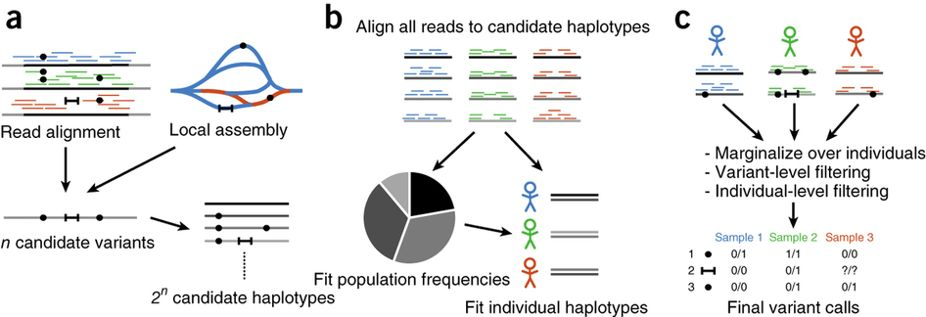
\includegraphics[scale=0.45]{platypus_main_flow}
    \centering
    \caption {Three stages of data processing in Platypus\autocite{rimmer2014integrating}}
    \label{fig:platypus_main_flow}
    \end{figure}


Platypus works by loading batches of reads into memory from a BAM file. 100 kb (kilobases) are loaded at a time. Low quality reads are filtered out. Sites that are flagged as potential variants by the aligned become candidate variants. The local assembly step operates on successive windows of 1.5 kb in size, including all reads that map to the window as well as their mates, irrespective of where or if they map. As a first step, the algorithm builds a colored de Bruijn graph\autocite{iqbal2012novo} from the reads and the reference sequence. Candidate variant haplotypes are produced by finding paths that diverge from the reference and come back to the reference by performing a Depth First Search from the graph node that diverges and until the reference is reached again. All such paths are recorded and contain putative SNPs, MNVs, indels, and larger rearrangements that are up to the window-size in length. A prior of $\num{0.33e-3}$ is used for SNPs under the assumption that SNPs occur in humans at a density of $10^{-3}$ per base and every non-reference allele is equally likely. Smaller windows are created by combining groups of candidate variants that are within 15 basepairs of each other, as long as window size is smaller than read-length and there are fewer than 8 variants in a group.

Candidate haplotypes are generated by taking all possible combinations of candidate variants (assuming diploid sample), resulting in  $2^n$ haplotypes. For a window with 8 variants there are 256 possible haplotypes. The haplotype likelihood $P(r|h)$ is calculated by aligning reads to each haplotype using a Hidden Markov Model. Platypus uses the Viterbi algorithm\autocite{forney1973viterbi} to compute the most likely path through the HMM as an approximation of the actual likelihood as a matter of optimization. After haplotype likelihoods are computed for all combinations of reads and haplotypes Platypus uses Expectation Maximization to estimate the frequency of each haplotype under the following model:

\begin{equation}
    \label{eq:platypus_likelihood_model}
    \mathcal{L}(R|\{h_i,f_i\}_{i=1 \dots a}) = \prod_{\substack{samples,\\ s}} \sum_{\substack{haplotypes,\\ i,j}} f_i f_j \prod_{\substack{reads,\\ r\in{R_s}}}\bigg(\frac{1} {2}{p(r|h_i)}+ \frac {1} {2}{p(r|h_j)}\bigg)
\end{equation}

where $f_i$ is frequency of haplotype $h_i$, $a$ is the number of considered alleles, $R$ is all reads, $R_s$ reads in sample $s$.

The posterior probability of a variant $v$ given the data is computed as:

\begin{equation}
    \label{eq:platypus_variant_posterior}
    P(v|R) = \frac {P(v)\mathcal{L}(R|\{h_i,f_i\}_{i=1\dots a})} {P(v)\mathcal{L}(R|\{h_i,f_i\}_{i=1\dots a}) + (1-P(v))\mathcal{L}(R|\{h_i,\frac{f_i}{1-F_v}\}_{i \in I_v})}
\end{equation}

here the likelihood of data $R$ given all haplotypes is compared to the likelihood of $R$ given those haplotypes that do not include $v$. $I_v$ is the set of haplotype indices such that $h_i$ does not contain $v$, and $F_v = \sum_{i \in I_v}f_i$. A variant is called when its posterior exceeds a pre-defined threshold. Genotype likelihoods for a variant are calculated by marginalizing over the genotypes at other variants within the window, and the best likelihood is selected as the genotype.

\subsubsection{Remarks}

Although samtools, freebayes, GATK, and Platypus are not the only tools that have been successfully used for germline SNP calling in the past 10 years, they have enjoyed sustained popularity and continued use in large scale genomics projects such as 1000 Genomes Project, ExAC\autocite{lek2016analysis}, PCAWG\autocite{stein2015data} and others. They thus can serve as primary examples of how the problem of calling germline SNPs is currently approached within the field, as well as providing a benchmark for new methods that attempt to solve similar problems. There are several key distinctions in the approaches that these tools take to the overall problem, yet a number of key similarities exist that we outline here and adopt as a general framework for tackling the SNP calling problem in our work.

\paragraph{Site Selection}

The problem of selecting sites in the genome for detecting variants has variety of approaches from evaluating every single site independently as one that potentially harbors a variant (as in samtools) to the varied windowing approaches used by the other variant callers. Looking at sites independently has the benefit of simplicity, while the windowing approach, at the expense of additional computation, allows a more comprehensive evaluation of a genomic region that is not limited to SNPs but can also support the detection of other types of variants. Thus, even though an independent site approach may be acceptable in an initial implementation, some form of windowing is desired in order to benefit from knowledge about the surrounding sequence context. In general, the interestingness of a site for the purposes of detecting a potential variant is universally linked to the presence of high quality reads spanning a particular locus that disagree with the reference sequence at that locus.

\paragraph{Haplotype Construction}

Samtools has the simplest model here as it does not attempt to construct haplotypes at all. This limits the ability of samtools to accurately represent genomic architecture, and prevents it from being able to supply phasing information for variants, which is of interest. Freebayes has the next simplest model, where putative haplotypes are constructed directly from the observed read sequences with the observation window. GATK and Platypus actually perform local assembly in the window to come up with an arrangement of reads that is free of artifacts\autocite{li2014towards} associated with alignment to the reference. Although local assembly appears to improve the ability of these callers to accruately represent sequence variants (especially non-SNPs) this processing step introduces a significant impact on the overall processing cost, mostly incurred from the resource-intensive HMM-aided alignment of reads to the putative haplotypes.

\paragraph{Allele Frequency Spectrum Estimation}

A distribution of allele frequencies in a population is of interest as it can be used as a prior in the calculation of genotype likelihoods for the samples under analysis and local and population-specific allele frequencies can vary significantly from values implied by generic population-genetics models. Most callers provide capabilities for estimating the Allele Frequency Spectrum by Expectation Maximization or similar approaches (Equation (5) in \autocite{li2011statistical}, not covered here, equation \ref{eq:freebayes_afs} for freebayes above). Alternatively, a non-informative prior (as in GATK) can be used.

\paragraph{Genotyping}

Pretty universally across the methods, genotyping is set up as a Bayesian inference selecting a Maximum Likelihood Estimate or a Maximum A Posteriori estimate of the genotype (for a single site or a haplotype) given the reads data, and taking into account the probability of errors dervied from read base quality and mapping quality scores supplied by the aligner. See Eq. \ref{eq:samtools_genotype} for samtools', Eq. \ref{eq:freebayes_main_model} frebayes', Eq. \ref{eq:gatk_genotyping} GATK's, Eq. \ref{eq:platypus_likelihood_model} Platypus' model setups. This model thus remains highly relevant for any new development in the space. 



\subsection{Germline Indel Calling}




\subsection{Germline Structural Variant Calling}
\label{sec:bg_germline_sv_calling}

Structural Variants (SVs) are medium- to large-size alterations (typically >50bp in length) of the genomic sequence that fall into a several broad categories (see Figure \ref{fig:sv_classes}) including insertions, deletions, tandem and interspersed duplications, inversions, translocations, mobile element insertions, as well as complex rearrangements that constitute a combination of the above classes or are otherwise difficult to classify. 

\begin{figure}[H]
    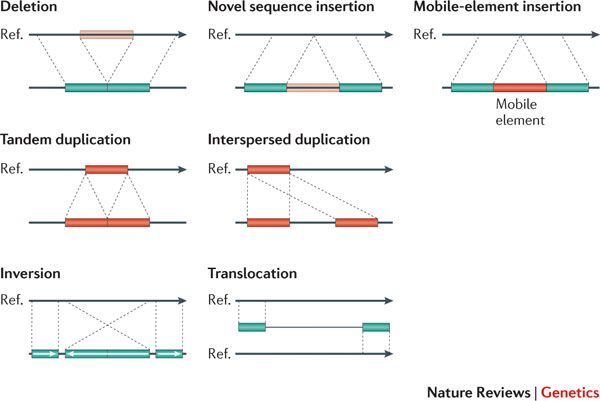
\includegraphics[scale=0.65]{sv_classes}
    \centering
    \caption {Classes of structural variation.\autocite{alkan2011genome}.}
    \label{fig:sv_classes}
\end{figure}

Accurate detection of SVs remains an open challenge since both sensitivity and specificity performance of SV calling is an order of magnitude worse than for SNP calling. For instance, in the latest data release of the 1000 Genomes Project an estimated sensitivity of 88\% was achieved for deletions, 65\% for duplications, 32\% for inversions\autocite{sudmant2015integrated} and False Discovery Rate of up to 89\%autocite{mills2011mapping}. A key challenge that impacts calling accuracy is small read size relative to the size of the variants. Since SVs can be hudreds of kilobases in length and typical Illumina reads are only 150-500 baspeairs long, accurate reconstruction relies on an agglomeration of reads in order to produce the variants. Structural Variant detection approaches typically make use of several sources of evidence (see Figure \ref{fig:sv_calling_info_sources}) for the detection of "breakpoints" - regions of the genome where a DNA double-strand break is detected and sequence is either inserted or excised. The breakpoints are then interpreted to produce the most likely variants that they represent. 

\paragraph{Discordantly-mapped read pairs} are pairs of sequencing reads that the alignment algorithm has mapped at a distance that is statistically significantly larger or smaller than the average read-pair distance for that sample, or that have an unusual read orientation, since read-pairs are supposed to be sequencing from two ends of a molecule towards each other. Reads that map closer than they are supposed to are indicative of an insertion, reads that map farther are indicative of a deletion, and reads that map in an unusual orientation are indicative of an inversion. 

\paragraph{Split-reads} are read-pairs where one of the reads maps properly but the aligner is not able to map the other read because different pieces of the read map to different locations in the genome indicating that this read spans a breakpoint. Distance between the split read pieces and their mapping orientation are informative of the type of breakpoint that the read spans.

\paragraph{Read-depth} Regions have a higher than normal or lower than normal read depth (count of reads spanning a region) are indicative of increased or reduced copy number respectively. Care must be taken to distinguish actual SVs from areas of repetitive sequence where the same simple sequence pattern is repeated many times. Typically aligners are not able to accurately resolve such areas and map many reads to the same set of coordinates making it appear like a duplication.

\paragraph{Assembly-based} approaches perform local assembly in a reference-free manner to reconstruct the variants encoded in the sample sequence that the aligner may struggle with resolving because of a large number or increased complexity of rearrangements.

\begin{figure}[H]
    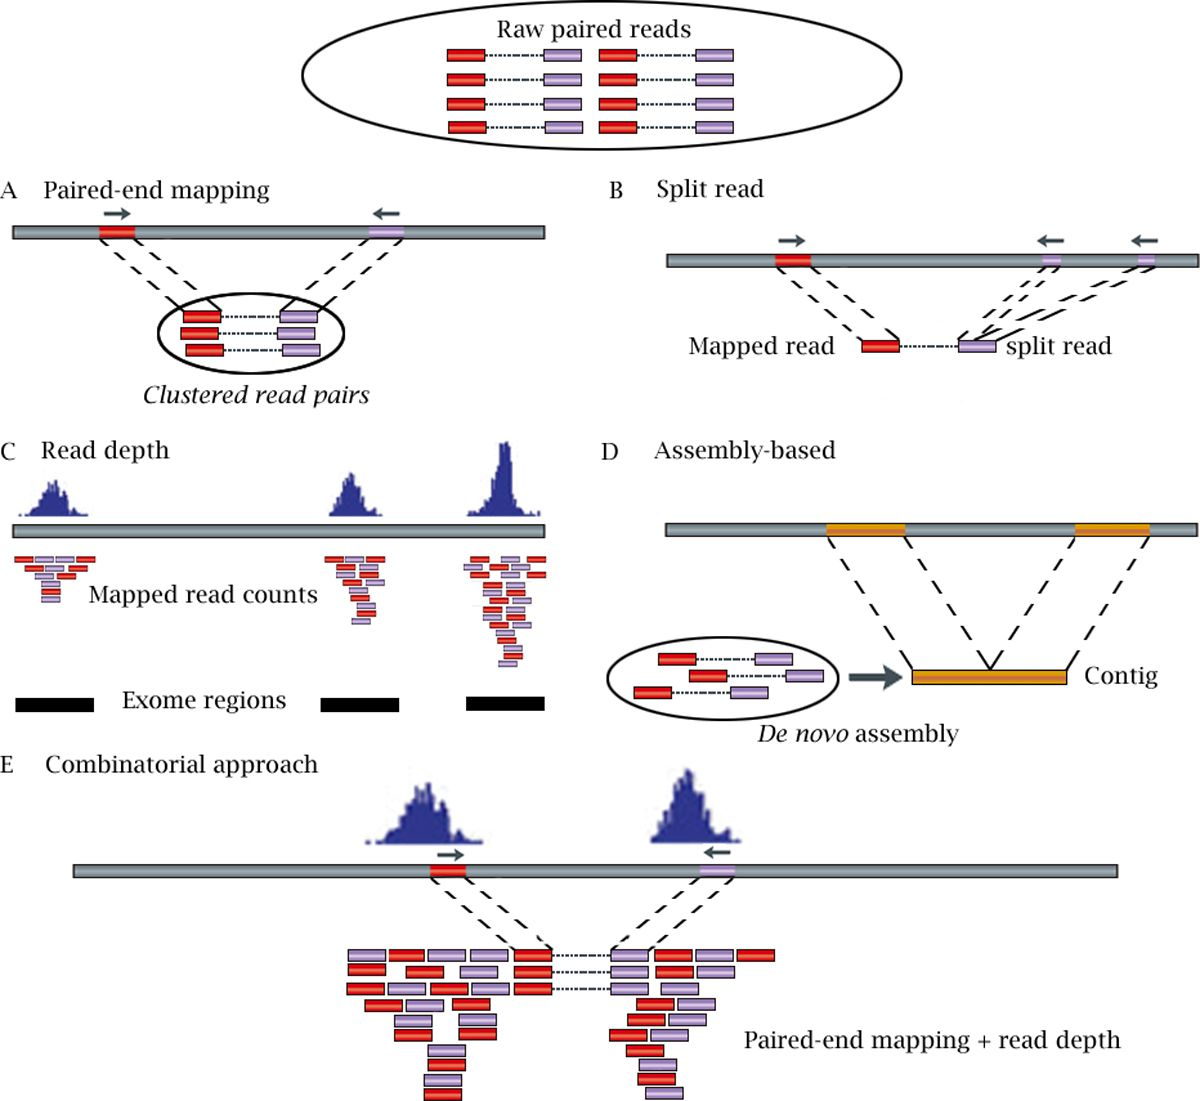
\includegraphics[scale=0.35]{sv_calling_info_sources}
    \centering
    \caption {Sources of evidence for the presence of Structural Variants.\autocite{zhao2013computational}.}
    \label{fig:sv_calling_info_sources}
\end{figure}

We look at several SV callers in closer detail.

\subsubsection{Delly}

Delly\autocite{rausch2012delly} is a structural variant calling tool built in 2011 by T. Rausch et al. in the context of the 1000 Genomes Project. Delly uses discordantly-mapped reads and split-reads as sources of evidence for the presence of SVs, is able to characterize a broad set of variants and has been implemented in C++. All of the mathematical formulas and figures in this section are reproduced from the 2012 mauscript by Raush et al.

The discordantly-mapped reads component of Delly begins by computing the median and standard deviation of the read insert size (distance between the ends of the two reads in a pair), as well as the default read orientation by sampling a pre-defined number of reads from the BAM file. Read-pairs that have an insert size farther than 3 standard deviations from the median are considered as evidence for structural variation. This induces a minimum SV size detectable by Delly. See Figure \ref{fig:delly_variant_classes} for the variant types implied by each insert size deviation and read-pair orientation.

\begin{figure}[H]
    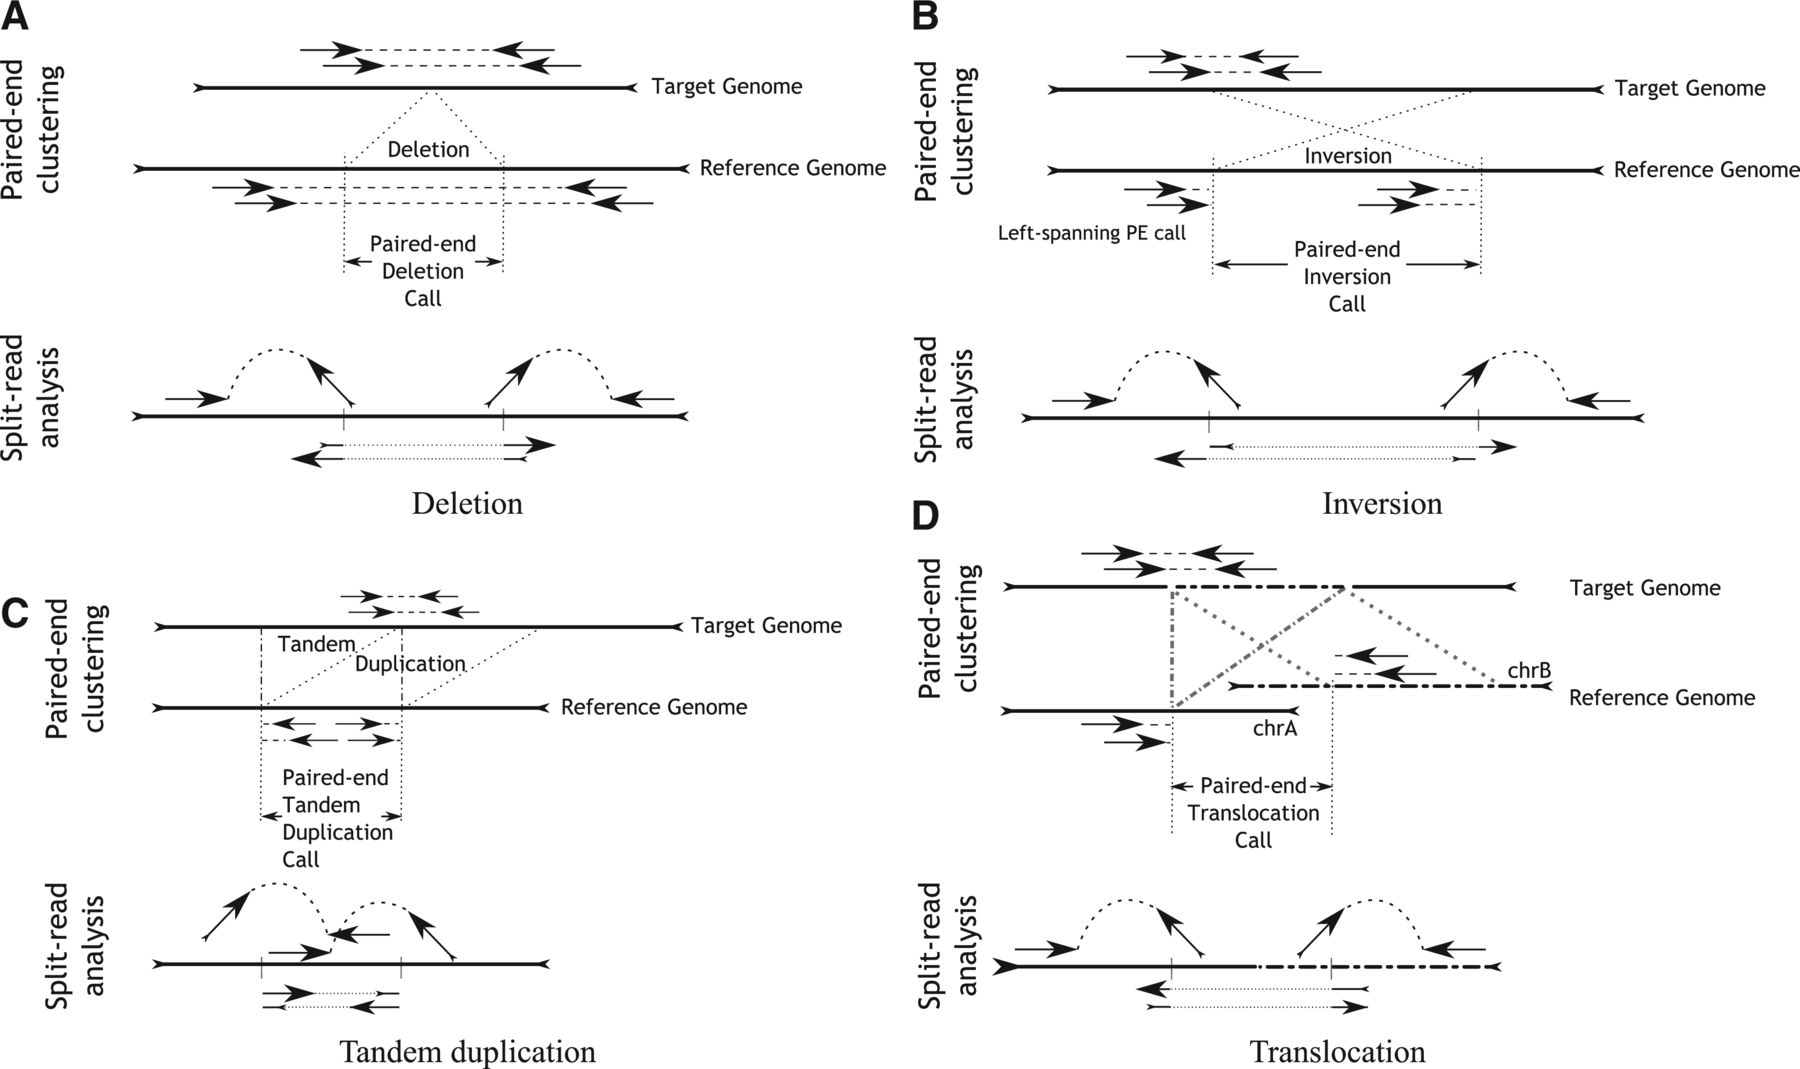
\includegraphics[scale=0.98]{delly_variant_classes}
    \centering
    \caption {Variant classes detectable by Delly based on their read-pair and split-read signatures.\autocite{rausch2012delly}.}
    \label{fig:delly_variant_classes}
\end{figure}

Using the list of discordantly-mapped read-pairs Delly builds an undirected, weighted graph to indicate which read-pairs support the same variant. In the graph $G(V,E)$, a read-pair $p_i$ corresponds to a node $v_i \in V$ and an edge $e_{v_i,v_j} \in E$ connects two nodes that support the same SV. The weight $w(e_{v_i,v_j})$ is the absolute value of the difference between the SV sizes predicted by $v_i$ and $v_j$. $v_i$ and $v_j$ support the same variant when the corresponding read pairs have the same read orientation and the absolute difference between the left and right ends of the two reads is less than the expected insert size. Variants are identified by computing connected components $C_i$ of $G$. When components are not fully connected, Delly sorts the edges in each such component by weight and attempts to find a maximal clique $M_i$ within $C_i$ using edge with the smallest weight as the seed of the clique. The clique is extended by searching for the next smallest edge for which one of the vertices is already in the clique $M_i$, and requiring that $M_i \cup \{v_l,v_m\}$ is also a clique, until no further vertices can be added. The vertices in $M_i$ are reported as the read pairs supporting that SV. Each rearrangement type is analyzed independently in this manner.

All of the rearrangements identified in the discordantly-mapped read analysis are refined using split-read analysis. The reads used for split-read analysis are those where one read in the pair maps to the reference and the other is unmapped. All such reads within a distance of 2 standard deviations of the median insert size from the breakpoint are considered up to a configurable maximum of 1000. Delly splits each unmapped read into kmers and aligns the kmers to the reference sequence spanning the SV.

\subsubsection{Lumpy}

Lumpy\autocite{layer2014lumpy} is an SV caller developed in 2013 by R. Layer et al. and is a package implemented in C++. All of the mathematical formulas and figures presented in this section are reproduced from the 2014 publication by R. Layer et al. 

\begin{figure}[H]
    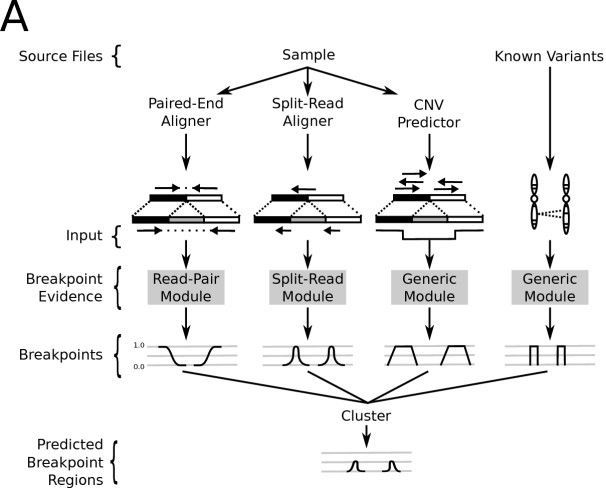
\includegraphics[scale=0.5]{lumpy_model}
    \centering
    \caption {Lumpy calling model integrates several signals from a single sample.\autocite{layer2014lumpy}.}
    \label{fig:lumpy_model}
\end{figure}

Lumpy defines an SV breakpoint as a pair of bases that are adjacent in the sample under study but not in the reference genome. Furthermore, each breakpoint is represented as a pair of probability distributions that span the predicted breakpoint regions and represent the uncertainty about the precise location of the breakpoint. Lumpy integrates multiple signals (see Figure \ref{fig:lumpy_model}) to update the probability distributions that represent each breakpoint based on different kinds of evidence provided. A breakpoint is a tuple $b = \langle E,l,r,v \rangle$ where $E$ is the evidence, $b.l$ and $b.r$ are the left and right intervals each having start and end coordinates, $b.l.s$ and $b.l.e$ for example. $b.l.p$ is a vector of length $b.l.e - b.l.s$ where each $p[i]$ is the probablity that $b.l.s + i$ is the true location of the breakpoint. $b.v$ is the breakpoint class (insertion, deletion, etc.). Overlapping breakpoints are merged together. The intervals that contain 95\% of the probability density, as well as the Maximum Likelihood Estimates of the location of each variant are returned. 

The paired-end analysis looks at read pairs $\langle x, y\rangle$ where each read is aligned to the reference genome as $R(x) = \langle c, o, s, e \rangle$ where $c$ is the chromosome, $o \in {+,-}$ indicates alignment orientation, $s$ and $e$ represent the alignment start and end respectively. It is assumed that $x$ and $y$ align uniquely and that $R(x).s < R(x).e < R(y).s < R(y).e$. $S(x) = \langle o, s, e \rangle$ is defined to be the alignment of $x$ with respect to the sample's (unknown) genome. Read pairs are assumed to be aligned with $R(x).o = +, R(y).o = -$ and having $R(y).e - R(x).s$ approximately equal to the library preparation fragment size. Read pairs that align outside the expected parameters for orientation and distance constitute evidence for structural variant breakpoints, in particular reads with the same or switched orientation, and pairs that align at a distance shorter or longer than the fragment size. Expected fragment length is estimated from the mean fragment length in the sample, along with its standard deviation. Breakpoint variety is determined as follows:

When $R(x).c = R(y).c$, the variety is inferred from read orientation. $R(x).o = R(y).o$ implies an inversion. $R(x).o = -, R(y).o = +$ implies a tandem duplication, $R(x).o = +, R(y).o = -$ implies a deletion. Insertions are not presently supported. When $R(x).c \ne R(y).c$ the breakpoint is labelled an interchromosomal rearrangement.

$\langle x, y \rangle$ are mapped to $b.l$ and $b.r$ as follows. By convention $x$ is assumed to map to $l$ and $y$ to $r$. It is assumed that there exists a single breakpoint $b$ between $x$ and $y$. Orientation of $x$ determines whether $l$ is upstream or downstream from $x$. Thus, if $R(x).s = +$, then the breakpoint begins after $R(x).e$. The length of the breakpoint interval is proportional to expected fragment length and its standard deviation. The distance of one end of the breakpoint from $x$ is assumed to be less than expected insert size $L$ plus $v_fs$ - a configurable number of standard deviations. The probability that position $i$ in the breakpoint interval $l$ is part of the actual breakpoint is estimated as the probability that $x$ and $y$ span $i$, which is true when the fragment that had produced $\langle x, y \rangle$ is longer than the distance from $x$ to $i$. Thus, the quantity of interest is $P(S(y).e - S(x).s > i - R(x).s)$ for $R(x).o = +$ and $P(S(y).e - S(x).s > R(x).e -i)$ for $R(x).o = -$. This quantity is estimated from the empirical distribution of fragment sizes collected from the sample.

Lumpy does not perform its own split-read alignment instead relying on the results of a split-read aligner like YAHA\autocite{faust2012yaha}. Every split-read is a DNA fragment $X$ that consits of two or more sub-fragments $x_i,...,x_j$ that do not map to adjacent locations of the reference. Each sub-fragment pair $\langle x_i, x_{i+1} \rangle$ is evaluated independently depending on how it maps with respect to the reference $R(x)$. When $R(x_i).o = R(x_{i+1}).o$ the event is marked as either a deletion or a tandem duplication, where $R(x_i).s < R(x_{i+1}).s$ implies a deletion, and otherwise a tandem duplication. When orientations do not match, the event is marked an inversion. To account for potential inaccuracies in the location of the breakpoint with respect to the split-read pair, each split-read pair is mapped to two breakpoint intervals $l$ and $r$ that are centered at the split. The probability is modeled to be highest at the split with an exponential decrease towards the edges, with a configurable width parameter.

\subsubsection{SvABA}

SvABA\autocite{wala2018svaba} is a germline and somatic SV caller by J. Walla et al., created in 2016. Svaba is implemented in C++ and relies on genome-wide local assembly for variant detection. Internally SvABA makes use of SGA\autocite{simpson2012efficient} and BWA-MEM\autocite{li2009fast} for assembly and read mapping respectively. 

\begin{figure}[H]
    \centering
    \caption {The SvABA variant callng method\autocite{wala2018svaba}.}
    \label{fig:svaba_method}
\end{figure}

SvABA performs local de-novo assembly in 25-kbp windows tiled across the genome with a 2kb overlap. First reads that may be indicative of variation are extracted from a BAM file, these include reads with high-quality soft-clipped bases, discordant reads (with non-standard orietnation or with insert size greater than four standard deviations away from the sample mean insert size, determined using a sample of 5 million reads with top and bottom 5\% of insert sizes truncated), unmapped reads, reads with unmapped mates, and reads with insertions or deletions indicated in the CIGAR string. Low quality reads that are marked as PCR duplicates, have failed QC, and reads with repeats of >20 basepairs are filtered out. Discordant reads are realigned to the reference with BWA-MEM and those with an available nondiscordant alignment of >70\% of the maximum alignment score are discarded. Reads with many different (>20) high quality candidate alignments are also discarded. Remaining discordant reads are clustered based on orientation and insert-size and assembled using SGA.

The contigs produced by SGA are aligned to the reference genome using BWA-MEM and examined for potential variants. Contigs with an alignment that has fewer than 30 nonaligned bases and no alignment gaps are considered reference. Indels are called when the alignment has gaps, and SVs called when the resulting alignment is multi-part. In order to evaluate read support for the putative variants, reads from the windows are aligned to both the reference and the assembled contigs using BWA-MEM. Reads are considered matching to the contig when the alignment score for the read to the contig is greater than the alignment of the read to the reference and is >90\% of the length of the match. Reads that have an alignment that is up to 8 bases to the left or right of a putative variant are consdered supporing the variant.

\subsubsection{Remarks}

We looked at Delly, Lumpy, and SvABA in the context of germline SV calling. Although there are some differences in the details of the approaches taken by the tools' authors there are consistent similarities as well, which additionally carry over to other SV callers such as Pindel\autocite{ye2009pindel}, and Manta\autocite{chen2015manta}, that have not been presented here. These approaches rely heavily on paired-end reads and select those that are mapped uncommonly far apart or close together. These are clustered or optionally locally assembled to produce putative breakpoints. Breakpoint locations are further refined by split-read analysis, using those reads that are unmapped by regular read mapping software. These reads are broken down into kmers and each kmer is aligned separately to non-adjacent locations in the genome. Alternative haplotypes may be constructed using these reads and alignments to the reference and the alternative haplotypes scored for genotyping purposes. A new method for structural variant calling should thus focus on making the best use of these two data types (discordant and split reads), while possibly also making use of read depth information to be competitive with the current generation of best callers. 

\subsection{Variant Filtering}

\subsection{Somatic SNP Calling}
Mutect - 
Muse - 
Pindel -


\subsection{Somatic Indel Calling}

\subsection{Somatic Structural Variant Calling}

\subsection{Germline Variant Annotation}
Annovar - 
Variant Effect Predictor - 


\subsection{Somatic Variant Annotation}

\subsection{de-novo Assembly}
Velvet -
Abyss - 

\section{High Performance , High Throughput, and Cloud Computing}

The practice of performing large scale scientific computation on supercomputers or clusters of commodity hardware can be split into two notions - High Performance Computing (HPC) and High Throughput Computing (HTC).

The European Grid Infrastructure defines these as follows\autocite{Glossary_V1_-_EGIWiki_2016-10-28}:

\fbox{\parbox[c]{0.9\textwidth}{HPC - A computing paradigm that focuses on the efficient execution of compute intensive, tightly-coupled tasks. Given the high parallel communication requirements, the tasks are typically executed on low latency interconnects which makes it possible to share data very rapidly between a large numbers of processors working on the same problem. HPC systems are delivered through low latency clusters and supercomputers and are typically optimised to maximise the number of operations per seconds. The typical metrics are FLOPS, tasks/s, I/O rates.}}

\fbox{\parbox[c]{0.9\textwidth}{HTC - A computing paradigm that focuses on the efficient execution of a large number of loosely-coupled tasks. Given the minimal parallel communication requirements, the tasks can be executed on clusters or physically distributed resources using grid technologies. HTC systems are typically optimised to maximise the throughput over a long period of time and a typical metric is jobs per month or year.}}

Although early High Performance Computing efforts (1960's - 1980's) relied on supercomputers with a shared memory model\autocite{russell1978cray}, where all of the memory was shared between multiple processors, by the late 1980's machines with a distributed memory model\autocite{nitzberg1991distributed}, where each processor has its own memory, started gaining ground, forming the basis for the modern HPC cluster.

The software interface that the user has to a HPC/HTC cluster typically takes the shape of a queueing system such as PBS\autocite{henderson1995job} or LSF\autocite{zhou1992lsf}  where the user writes a script that submits a series of jobs to the queueing system. The jobs can invoke software that is installed by the IT department that manages the cluster. The user is not able to install any software and has limited visibility into the runtime performance characteristics of the jobs they submit. 

Cloud computing has emerged in the early 2000's enabled by improvements in hardware virtualization which was driven by the adoption of Virtual Private Networks, and the desire to commercialize access to compute capacity as a utility\autocite{buyya2009cloud}.

The National Institute of Standards and Technology provides a standard definition of cloud computing that encompasses several areas of this domain - Essential Characteristics, Service Models, and Deployment Models\autocite{mell2011nist}.

The Essential Characteristics of a cloud are as follows:

\begin{description}
\item [On-demand self-service] - End-user can independently manage infrastructure without involving the service provider.
\item [Broad network access] - Cloud resources are available on the network via a set of standard protocols.
\item [Resource pooling] - Service providers dynamically assign virtual infrastructure in a multi-tenant environment based on consumer demand.
\item [Rapid elasticity] - Resources can be elastically provisioned and discarded according to customer requirements.
\item [Measured service] - Resource usage by end users is measured and transparently provided back to the user by the service provider.
\end{description}

It is the self-service and broad network access characteristics that set cloud computing apart from traditional HPC computing the most.

Service Models include:

\begin{description}
\item [Infrastructure as a Service (IaaS)] - This service allows the the user to provision and control virtualized infrastructure such as VMs and networks.
\item [Platform as a Service (PaaS)] - This service allows the user to deploy their application onto virtualized hardware but not to control the management of the infrastructure.
\item [Software as a Service (SaaS)] - This service allows the user to make use of applications that are deployed on virtualized hardware but not to manage the applications or the infrastructure itself.
\end{description}

The Deployment Models covered by the NIST definition are as follows:

\begin{description}
\item [Private Cloud] - Operated privately by a single organization and not accessible on a public network.
\item [Community Cloud] - Established for use by a particular community of users with a common interest.
\item [Public Cloud] - Established for general use by the public.
\item [Hybrid Cloud] - A collection of cloud entities that use one of the other deployment models but allow application portability.
\end{description}

The first publicly available commercial cloud computing platform has been developed by Amazon.com and launched in August, 2006 in the form of two services - Elastic Compute Cloud (EC2), and Simple Storage Service (S3). Cloud offerings by Microsoft and Google followed in 2010, and 2012. This early lead has allowed Amazon to capture the majority of the public cloud computing market, earning \$2.57 billion USD in Q1 2016 revenue.

One of the main drawbacks, however, of using Amazon's or another proprietary cloud solution is the issue of "vendor lock-in" i.e. inability to easily switch infrastructure providers should the customer wish to do so, because of the amount of software relying on the proprietary cloud provider protocols. Another key reason for avoiding public clouds is the necessity to store sensitive data. This issue applies both to the commercial enterprise (with industries such as banking, and payments) and scientific domains (especially genomics and medicine) where handling of sensitive patient data is restricted based on both technical security, as well as ethical considerations\autocite{knoppers2005human}.

To help alleviate these concerns an open-source cloud platform called Openstack was launched in 2010 jointly by Rackspace Hosting and NASA\autocite{sefraoui2012openstack}. Openstack provides most of the same features that are provided by Amazon Web Services and other commercial cloud providers as free open-source tools. These include:

\begin{itemize}
\item Infrastructure
\item Networking
\item Identity Management
\item Block Storage
\item Object Storage
\item Managed Databases
\item Queues
\item Monitoring
\end{itemize}

Openstack deployments for the basis for most academic private and community clouds such as EBI Embassy Cloud\autocite{cook2016european}, University of Chicago Open Science Data Cloud\autocite{grossman2010overview}, Cancer Genome Collaboratory\autocite{yung2016icgc}, and Helix Nebula\autocite{marx2013biology}. Because these clouds implement the security measures necessary when handling patient data they are a system of choice for large scale bioinformatics analyses.

\section{Workflow Systems}

The focus on workflow stems the work of Frederick Taylor (1856-1915) and Henry Gantt (1861-1919) on the improvement and automation of industrial processes, also known as "scientific management"\autocite{taylor2004scientific}. One of the key techniques that were devised at the time and served as the prototype for future workflows were "time and motion studies"\autocite{barnes1949motion} where employees were observed as they performed repetitive cycles of work in order to determine standard execution times and sequences of steps. As this field evolved over the course of the 20th century it gave rise to several other related fields such as Operations Management, Business Process Management, and Lean Manufacturing.

In 1993 an international consortium was formed with the purpose of defining the standards related to workflows and workflow management systems. This consortium is called the Workflow Management Coalition (WfMC). One of the key specifications produced by the WMC in 1995 is The Workflow Reference Model\autocite{hollingsworth1995workflow}. This document provides two basic definitions that illuminate the scope and purpose of  workflow systems:

\fbox{\parbox[c]{0.9\textwidth}{Workflow - The computerised facilitation or automation of a business process, in whole or part.}}

\fbox{\parbox[c]{0.9\textwidth}{Workflow Management System - A system that completely defines, manages and executes "workflows" through the execution of software whose order of execution is driven by a computer representation of the workflow logic.}}

A number of standards have been produced for workflow definition, many of them are XML-based\autocite{shapiro2002technical}. Notable examples include:

\begin{description}
\item[XPDL] - Was developed by the WfMC, currently at version 2.2, as of 2012. Uses an XML dialect to express process definitions
\item[BPML] - Developed by the Object Management Group (OMG) using XML. Deprecated as of 2008 in favour of BPEL.
\item[BPEL/BPEL4WS] -  Developed by Organization for the Advancement of Structure Information Standard (OASIS). Uses XML format. Adopted by Microsoft and IBM for their workflow products - 
\end{description} 

Graphically, workflow definitions are typically expressed using a Petri-Net\autocite{peterson1981petri} or Business Process Model and Notation (BPMN), the latter borrowing its structure from UML activity diagrams. A set of workflow definition design patterns exists to guide workflow creation\autocite{van2003workflow}. A workflow engine is responsible for ingesting workflow definitions, generating their graphical representation, and allowing the user to execute the workflow definitions on suitable hardware.

As initially the focus of workflow systems research and development has been on process improvement within commercial enterprises there exists a large pool of workflow engine implementations targeted at that sector. Some of these are:

\begin{description}
\item[jBPM] - An open-source workflow engine that is based on the Java platform and is currently owned by Red Hat.
\item[Activiti] - An open-source workflow engine that has been developed by previous jBPM developers.
\item[Oracle BPEL Process Manager] - A commercial workflow engine acquired by Oracle from Collaxa in 2004, now integrated into the rest of the Oracle portfolio.
\item[Websphere Process Server] - Commercial workflow engine that is part of IBM's Business Process Manager suite.
\end{description}

Although these tools have gained wide adoption in the enterprise community they have had limited success within scientific circles. Instead, several open-source workflow management systems exist that have been purpose-built for the scientific domain, and especially bioinformatics. These include:

\begin{description}
\item[Kepler\autocite{ludascher2006scientific}] - A Java-based WfMS built on top of the Ptolemy II\autocite{davis1999overview} execution engine.
\item[Taverna\autocite{oinn2004taverna}] - A Java-based WfMS originally built by myGrid, currently under incubation at Apache Software Foundation. 
\item[Galaxy\autocite{goecks2010galaxy}] - A Python-based WfMS developed specifically for bioinformatics applications with a focus on GUI-driven development of workflows.
\end{description}

Curcin et al\autocite{curcin2008scientific} provide a head-to-head comparison of six scientific workflow systems including Taverna and Kepler, whereby Taverna is described as primarily being aimed at researchers who wish to build scientific workflows from web services utilizing a proprietary XML dialect called SCUFL which implements a DAG model of workflows. The primary execution environment for a Taverna workflow is on a grid or an HPC cluster. Kepler implemented a different methodology, whereby workflow modelling, which is taken on by Actors, is separated from workflow execution, taken on by Directors. An Actor knows only about its inputs, the computation that it needs to perform, and the output that it needs to produce, while Directors provide different models of execution, such as Synchronous Data Flow, Process Network, Continuous Time, and Discrete Event.

The Galaxy workflow framework has a specific focus on bioinformatics analyses and comes with a large library of community-developed bioinformatics workflows. The user creates and executes workflows via a web-based GUI where pre-installed tools and scripts can be laid out into a pipeline. The primary deployment environment for Galaxy is on an institutional HPC cluster although a separate component allows the deployment of a Galaxy instance on Amazon Web Services\autocite{afgan2010galaxy}.

\section{Service Oriented Architectures}

\section{Stream-based Systems}

